% v0.3 (2026-10-02): bounded C7 diagram alignment and current series scope; historical definitions and raw audit codes retained.
% Bridge_Contract_Criterion_v0_en.tex — Gap Series Part 2 (EN)
% Status: v0.2 MAJOR REVISION (2026-08-16) — built strictly to the healer
% blueprint of the 3-agent review round 1
% (_results/3agenten_review/Teil2_BridgeContract_HEILER_2026-08-16.md, §§3–9)
% as ruled by _results/3agenten_review/Teil2_BridgeContract_RICHTER_2026-08-16.md.
% v0.2 changes: instrument versioning v1-F / v1-T with T-/F- namespacing;
% Components 6 and 7 hardened (mandatory compatibility identities; addressed
% order lemma with H1–H5; explicit auditor boundary); ledger replaced by the
% normative crosswalk (F-R6a/F-R6b split, F-R4a/F-R4b -> C5, F-R8 as E8 with
% default X); calibration relabelled as a protocol-frozen retrospective
% two-case illustration of v1-T with the full dissent matrix; abc findings
% reweighted (F-R2a = X, no artificial C6 pass, multiple weighted findings);
% Joshi = comparative discrimination case, Prasad the only accepted control;
% LANA = external point of comparison; scope reduced to ONE abc instantiation
% plus RH/global-only outlook; AI disclosure wired in; operator blocks moved to
% _claude-work/T2_REMOVED_COMMENTS_2026-08-16.md.
% v0.1 lineage: structure approval D-005=A [U 2026-08-15]; P0 gates G1–G5
% discharged; sec:related from t2-s3 (crosswalk), sec:abc from t2-s4;
% sec:calibration from the protocol-frozen two-case audit
% (BCM_AUDIT_SYNTHESE_V1). T2-BIB integrated 2026-08-16 (36 verified entries,
% 0 undefined citations; prasad pages corrected 91–114 at the primary
% document). Open before upload: retest refuter, DE translation, dry-run,
% supplement of per-row anchor tables (P1-5). No kombi (convention 2026-08-15).
\documentclass[11pt,a4paper]{article}
\usepackage{cmap}
\usepackage[utf8]{inputenc}
\usepackage[T1]{fontenc}
\usepackage{lmodern}
\usepackage{microtype}
\usepackage{amsmath,amssymb,amsthm}
\usepackage{booktabs}
\usepackage{tabularx}
\usepackage{tikz}
\usetikzlibrary{arrows.meta,positioning,shapes.geometric,fit,calc}
\usepackage[colorlinks=true,linkcolor=blue,citecolor=blue,urlcolor=blue]{hyperref}
\usepackage{xurl}
\hypersetup{
  pdfencoding=unicode,
  psdextra,
  breaklinks=true,
  pdflang={en-US},
  bookmarksnumbered=true,
  bookmarksopen=true,
  pdfpagemode=UseOutlines,
  pdftitle={The Bridge-Contract Criterion: A Form Audit for Transport Arguments, with an Instantiation in the abc Literature},
  pdfauthor={Lukas Geiger},
  pdfsubject={Proof Auditing, Bridge Contract, Transport Arguments, abc Conjecture},
  pdfkeywords={abc conjecture, proof auditing, transport arguments, bridge contract, ledger audit, Mochizuki, Joshi}
}
\renewcommand*{\HyperDestNameFilter}[1]{en.#1}
\input{glyphtounicode}
\pdfgentounicode=1

% Typographic penalty guards and spacing
\clubpenalty=10000
\widowpenalty=10000
\displaywidowpenalty=10000
\setlength{\emergencystretch}{1.5em}
\hyphenation{Teich-mül-ler Teich-mul-ler}

\newtheorem{definition}{Definition}[section]
\newtheorem{lemma}{Lemma}[section]
\newtheorem{remark}{Remark}[section]

\title{The Bridge-Contract Criterion:\\A Form Audit for Transport Arguments,\\with an Instantiation in the abc Literature}
\author{Lukas Geiger\\\small Independent Researcher, Bernau, Germany\\\small ORCID: 0009-0005-7296-1534}
\date{October 2026 --- version 0.3}

\begin{document}
\maketitle

\begin{abstract}
Some proof claims resist line-by-line review not because individual steps are
opaque, but because their load-bearing core is a \emph{transport}: a quantity
migrates between theoretical frameworks, and the claim's numerical content rests
on the admissibility of that migration. A related class rests on
\emph{global-only} statements: assertions available only after summation over all
places, with no place-wise access. We propose a seven-component bridge contract
and a versioned ledger audit. We report a retrospective two-case feasibility
illustration of the frozen v1-T transport ledger and one substantive
selected-rows instantiation of the criterion in the abc literature (the
v1-F rows exercised there are named; the full-matrix coding of all rows is
deferred). The paper contains no
RH-side verdict; RH uniformity and global-only positivity claims are retained as
an explicitly untested outlook. The criterion judges contract \emph{form}, not
mathematical truth: a served ledger is necessary, not sufficient, and the auditor
tests the presence and addressability of an obligation, never its mathematical
validity. Its value is that failures localize --- the audit names the missing
clause at a stated row instead of a diffuse doubt.
The current research state aligns the conditional C7 illustration with all five
hypotheses of the unchanged contract definition, after a counterexample to the
earlier incomplete diagram. Later developments in Parts 4--6 are distinguished
from the historical audit pins: same-field rigidity permits global scaling,
while coordinate, field, period and volume bridges remain open. The two-case
raw matrix remains a version-scoped illustration, not a reliability estimate.
\end{abstract}

\clearpage
\tableofcontents
\clearpage

%=====================================================================
\section{Introduction}\label{sec:intro}

Two classes of proof claims resist classical line-by-line review in a
characteristic way. The first are \emph{transport claims}: a quantity is
constructed in one framework and its numerical reading is asserted to land in
a target region fixed in another, with the claim's content resting on the
admissibility of the migration rather than on any single computational step.
The documented precedent is the disputed transport step of Mochizuki's
Corollary 3.12, whose ten-year controversy consists, on our reading, not of
disagreement about individual lines but of disagreement about what the
transport \emph{owes}~\cite{part1}. The second are \emph{global-only
claims}: assertions available only after summation over all places, with no
place-wise access --- a shape that occurs both in the abc literature and in
positivity approaches to the Riemann Hypothesis.

This paper proposes a checkable form criterion for both classes: the
\emph{bridge contract}, a list of seven contract components that a
transport must serve before its numerical conclusion may be drawn, together
with a ledger-style audit protocol with a fixed verdict grammar. The
criterion grew out of the audits of this series --- the gap localization of
Part 1~\cite{part1} and the certificate instrument of Part 3~\cite{part3}
--- and has since been applied, in the later parts, to the principal
published repair program~\cite{part4,part5,part6}. Here we present the
criterion itself as a transferable method: its definition
(Section~\ref{sec:criterion}), its position among existing auditing
structures (Section~\ref{sec:related}), a protocol-frozen retrospective
two-case illustration of the frozen transport ledger
(Section~\ref{sec:calibration}), and one selected-rows instantiation of the
criterion on the abc transport step (Section~\ref{sec:abc}). The
companion landscape paper of the program records how the criterion sits
among the routes it audits~\cite{landscapeA}.

Two limits of scope are stated here rather than left to be inferred. First,
the instrument is \emph{versioned}: the full ledger of
Section~\ref{sec:ledger} and the six-row transport ledger used for the
retrospective illustration are two distinct instruments with a published
crosswalk, and identical numeric row suffixes do not imply identical
semantics. Second, this paper reports exactly one instantiation, in the abc
literature, and that instantiation is \emph{selected-rows}: the rows
exercised are named in Section~\ref{sec:abc}, and a coding of the complete
v1-F matrix for these cases is deferred to a later version. By an
\emph{instantiation} we mean throughout the application of the criterion to
one dispute complex --- here the abc transport dispute, comprising the
original argument and its repair program as a single complex with two
audited profiles. Uniformity claims toward the Riemann
Hypothesis and global-only positivity claims appear as an explicitly
untested outlook (Sections~\ref{sec:rh} and~\ref{sec:global}); no RH-side
verdict is drawn anywhere below.

To keep the counting unambiguous, the cases treated in this paper are named
by kind and not by ordinal throughout: a \emph{retrospective known-gap
case} and an \emph{accepted control} (Section~\ref{sec:calibration}), the
\emph{abc instantiation} with a \emph{comparative discrimination case} and
a \emph{downstream inheritance example} (Section~\ref{sec:abc}), an
\emph{external comparison} (Section~\ref{sec:abc-external}), and the
\emph{RH / global-only outlook} (Sections~\ref{sec:rh} and~\ref{sec:global}).

Throughout, one boundary is maintained without exception: the criterion
judges \emph{contract form}, not mathematical truth. A fully served ledger
is necessary for the admissibility of a transport reading, never sufficient
for the underlying claim; an unserved row localizes an obligation, it does
not refute a theorem. The auditor tests whether an obligation is present
and addressable in a named version of a text, never whether the mathematics
it names is correct. The value we claim for the method is exactly this
localization: audits that end in a named missing clause rather than a
diffuse doubt.

%=====================================================================
\section{The Criterion}\label{sec:criterion}

\subsection{The Bridge Contract}\label{sec:contract}

The situation we axiomatize is the following. A proof asserts a numerical
conclusion of the form ``the reading of an object constructed in framework $A$
lands in a target region fixed in framework $B$'', where the two frameworks do
not share a common evaluation by construction. The assertion is mediated by a
\emph{transport}: labels, containers, or functors that relate the two sides.
The criterion asks what the transport must \emph{contractually} provide before
the numerical conclusion may be drawn.

\begin{definition}[Bridge contract]\label{def:bridge}
Let a claim relate a source object to a numerical target region. A
\emph{bridge contract} $\mathrm{Br}$ for this claim consists of the following
seven components.
\begin{enumerate}
  \item \textbf{Source object with readout} ($X_q$, $\nu_q$, $i_q$): the
    source-side domain $X_q$, a concrete numerical readout functional
    $\nu_q\colon X_q \to V$ into the ordered value space of Component~2, and
    the typed map $i_q\colon X_q \to C$ into the container of Component~3 (in
    the motivating case: a log-volumetric reading of the $q$-pilot).
  \item \textbf{Target object with target readout and fixed target region}
    ($X_\Theta$, $\nu_\Theta$, $(V,\preceq)$, $H_\Theta$): the target
    domain $X_\Theta$, a target readout $\nu_\Theta\colon X_\Theta \to V$, an
    ordered value space $(V,\preceq)$ shared by both readouts, and a target
    region $H_\Theta \subseteq V$ fixed \emph{in advance} --- a lower set
    $H_\Theta = \{v \in V : v \preceq \tau_\Theta\}$ or the corresponding
    upper set, with the threshold $\tau_\Theta \in V$ named before the source
    value is inspected. The typed map $i_\Theta\colon X_\Theta \to C$ belongs
    to Component~3. In the motivating case $V = \mathbb{R}$ with its usual
    order and $H_\Theta = \mathbb{R}_{\le -|\log\Theta|}$.
  \item \textbf{Typed common container} ($C$, $\preceq_C$,
    $i_q\colon X_q \to C$, $i_\Theta\colon X_\Theta \to C$): a common
    receptacle equipped with the order relation $\preceq_C$ used by the
    claim (a partial order, or the preorder the source itself specifies,
    stated with its carrier), together with \emph{explicitly typed} maps
    from both sides, each given with its domain and codomain. A container in
    which both objects merely cohabit does not by itself carry scale, and a
    container without a stated order carries no order claim.
  \item \textbf{Admissible linkage} ($L$): label or linkage data that specify
    an \emph{allowed identification}, not mere homonymy. Sharing a name across
    frameworks is not a mathematical relation.
  \item \textbf{Separated indeterminacy budget} ($I$): an explicit budget
    distinguishing absorbable renormalization, blurring, and
    \emph{non-absorbed residual load}. An indeterminacy that is invoked to
    absorb an obstruction must be booked against this budget, not against the
    container.
  \item \textbf{Compatible common evaluation} ($\nu_C$). A typed map
    $\nu_C\colon C\to(V,\preceq)$ is supplied together with the compatibility
    identities required by the claim, in particular $\nu_C\circ i_q=\nu_q$ on
    the stated source domain and, where the target is represented by a target
    readout $\nu_\Theta$, $\nu_C\circ i_\Theta=\nu_\Theta$ on the stated target
    domain. These compatibility clauses are mandatory; the mere existence of a
    numerical map on $C$ never discharges this component.
  \item \textbf{Addressed order lemma.} A named lemma states the hypotheses
    under which the admissible linkage yields an order relation in $C$, states
    the monotonicity and target-region hypotheses, and derives the required
    target membership. For a lower target set
    $H_\Theta=\{v\in V:v\preceq\tau_\Theta\}$, a typical form is: if (H1)
    $L(x,y)$ is admissible, (H2) $i_q(x)\preceq_C i_\Theta(y)$, (H3) $\nu_C$ is
    monotone on such linked pairs, (H4) the compatibility clauses of
    Component~6 hold, and (H5) $\nu_C(i_\Theta(y))\preceq\tau_\Theta$, then
    $\nu_q(x)\in H_\Theta$. Hypothesis (H2) is never a free assumption: the
    contract requires the text either to \emph{derive} it from the linkage
    data of Component~4 in an addressed sublemma, or to prove it separately
    --- in both cases with its own proof address. The same anchoring
    requirement applies to every load-bearing hypothesis of the lemma.
\end{enumerate}
\end{definition}

A contract audit records this component as textually served only when the
lemma, its hypotheses, its claimed applicability at the audited step, and a
proof address are present and inspectable in the named version. The auditor
tests presence and addressability, not mathematical validity. A served row
therefore does not certify that the lemma or its proof is correct.

Components 6 and 7 are the load-bearing clauses: without them, common-container
cohabitation together with shared labels yields only qualitative nearness. In
the precedent cases audited below they are also where the heaviest findings
fall --- but not the only rows that carry findings, and the ledger reports the
full profile rather than a single surviving row.

Figure~\ref{fig:bridge_contract_architecture} illustrates the conceptual architecture of a bridge contract, mapping the interaction of the seven canonical components between the disjoint source and target frameworks. Table~\ref{tab:contract_components} summarizes the seven canonical components, their mathematical signatures, the required verification obligations, and the characteristic failure modes.

\begin{figure}[htbp]
\centering
\resizebox{0.98\textwidth}{!}{%
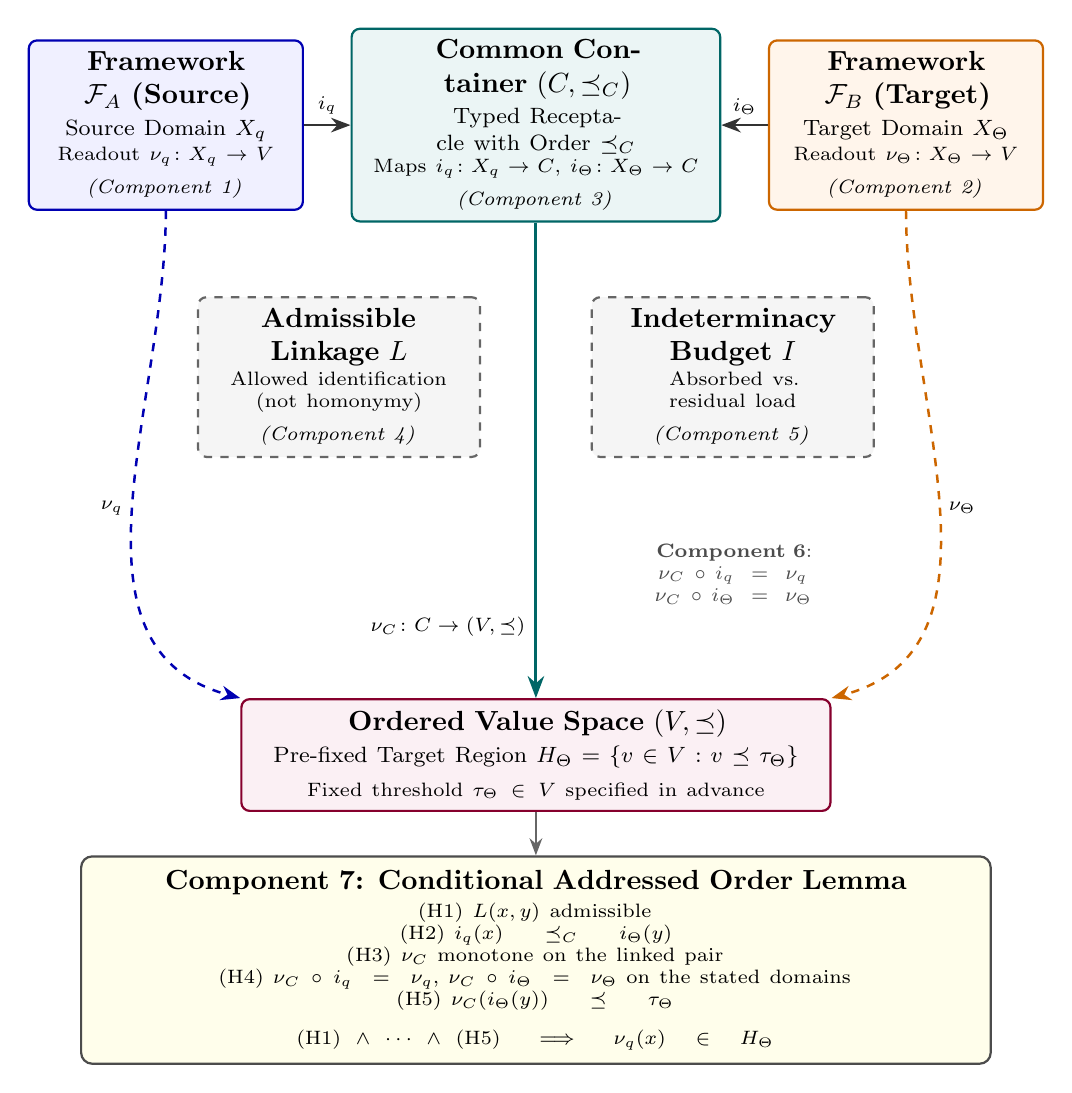
\begin{tikzpicture}[
  >=Stealth,
  box/.style={draw=black!70, rounded corners=3pt, line width=0.8pt, align=center, inner sep=4pt},
  srcbox/.style={box, fill=blue!6, draw=blue!70!black},
  tgtbox/.style={box, fill=orange!8, draw=orange!80!black},
  ctrbox/.style={box, fill=teal!8, draw=teal!80!black},
  valbox/.style={box, fill=purple!6, draw=purple!70!black},
  gatebox/.style={box, fill=gray!8, draw=black!60, dashed},
  arrow/.style={->, line width=0.9pt, draw=black!80},
  annot/.style={font=\scriptsize, text=black!70, align=left}
]

  % Top layer: Source, Container, Target
  \node[srcbox, text width=3.2cm] (src) at (0, 7.0) {
    \textbf{Framework $\mathcal{F}_A$ (Source)}\\[2pt]
    \footnotesize Source Domain $X_q$\\[1pt]
    \scriptsize Readout $\nu_q\colon X_q \to V$\\
    \textit{(Component 1)}
  };

  \node[ctrbox, text width=4.4cm] (ctr) at (4.7, 7.0) {
    \textbf{Common Container $(C, \preceq_C)$}\\[2pt]
    \footnotesize Typed Receptacle with Order $\preceq_C$\\
    \scriptsize Maps $i_q\colon X_q \to C$, $i_\Theta\colon X_\Theta \to C$\\
    \textit{(Component 3)}
  };

  \node[tgtbox, text width=3.2cm] (tgt) at (9.4, 7.0) {
    \textbf{Framework $\mathcal{F}_B$ (Target)}\\[2pt]
    \footnotesize Target Domain $X_\Theta$\\[1pt]
    \scriptsize Readout $\nu_\Theta\colon X_\Theta \to V$\\
    \textit{(Component 2)}
  };

  % Intermediate layer: Linkage and Budget
  \node[gatebox, text width=3.3cm] (link) at (2.2, 3.8) {
    \textbf{Admissible Linkage $L$}\\[1pt]
    \scriptsize Allowed identification (not homonymy)\\
    \textit{(Component 4)}
  };

  \node[gatebox, text width=3.3cm] (bdg) at (7.2, 3.8) {
    \textbf{Indeterminacy Budget $I$}\\[1pt]
    \scriptsize Absorbed vs.\ residual load\\
    \textit{(Component 5)}
  };

  % Value Space
  \node[valbox, text width=7.2cm] (val) at (4.7, -1.0) {
    \textbf{Ordered Value Space $(V,\preceq)$}\\[2pt]
    \footnotesize Pre-fixed Target Region $H_\Theta = \{v \in V : v \preceq \tau_\Theta\}$\\
    \scriptsize Fixed threshold $\tau_\Theta \in V$ specified in advance
  };

  % Embeddings
  \draw[arrow] (src.east) -- (ctr.west) node[midway, above, font=\scriptsize] {$i_q$};
  \draw[arrow] (tgt.west) -- (ctr.east) node[midway, above, font=\scriptsize] {$i_\Theta$};

  % Downward evaluation
  \draw[arrow, line width=1.1pt, draw=teal!80!black] (ctr.south) -- (val.north)
    node[pos=0.85, left, font=\scriptsize] {$\nu_C\colon C \to (V,\preceq)$};

  \node[annot, text width=3.8cm, align=center] at (7.2, 1.3) {
    \textbf{Component 6}:\\
    $\nu_C \circ i_q = \nu_q$\\
    $\nu_C \circ i_\Theta = \nu_\Theta$
  };

  % Direct readouts to value space
  \draw[arrow, dashed, draw=blue!70!black] (src.south) to[out=-90,in=165]
    node[left, font=\scriptsize] {$\nu_q$} (val.north west);
  \draw[arrow, dashed, draw=orange!80!black] (tgt.south) to[out=-90,in=15]
    node[right, font=\scriptsize] {$\nu_\Theta$} (val.north east);

  % C7: north anchor below the value node; extra hypotheses grow down.
  \node[draw=black!70, rounded corners=4pt, line width=0.8pt, fill=yellow!8,
    text width=11.2cm, align=center, inner sep=5pt, anchor=north]
    (lem) at ($(val.south)+(0,-0.55)$) {
    \textbf{Component 7: Conditional Addressed Order Lemma}\\[2pt]
    \scriptsize (H1) $L(x,y)$ admissible\\
    \scriptsize (H2) $i_q(x)\preceq_C i_\Theta(y)$\\
    \scriptsize (H3) $\nu_C$ monotone on the linked pair\\
    \scriptsize (H4) $\nu_C\circ i_q=\nu_q$, $\nu_C\circ i_\Theta=\nu_\Theta$ on the stated domains\\
    \scriptsize (H5) $\nu_C(i_\Theta(y))\preceq\tau_\Theta$\\[2pt]
    \scriptsize $(\mathrm{H1})\land\cdots\land(\mathrm{H5})\ \Longrightarrow\ \nu_q(x)\in H_\Theta$
  };

  \draw[arrow, draw=black!60, line width=0.7pt] (val.south) -- (lem.north);

\end{tikzpicture}%
}
\caption{Conditional bridge-contract illustration for the lower target set. All
five hypotheses are required; (H2) and every load-bearing obligation need
their own proof addresses. The diagram illustrates the contract and does
not certify the correctness of a source proof.}
\label{fig:bridge_contract_architecture}
\end{figure}

\paragraph{Development of the C7 illustration.}
The earlier diagram omitted the target bound (H5) and replaced compatibility
(H4) by a bounded residual load. Its implication fails in the identity model:
take every domain and carrier to be $\mathbb R$, every displayed map to be the
identity, the usual order, $x=y=1$, admissible $L(x,y)$, residual load $0$,
$\tau_\Theta=0$, and $H_\Theta=(-\infty,0]$. The earlier displayed premises
hold, including compatibility, but $\nu_q(x)=1\notin H_\Theta$. This refutes
the incomplete diagram implication, not Definition~\ref{def:bridge} with
(H1)--(H5). Figure~\ref{fig:bridge_contract_architecture} now displays those
five conditions separately; the illustration does not certify a source proof
or establish experimental validation of the method.



\begin{table}[htbp]
\centering
\footnotesize
\renewcommand{\arraystretch}{0.95}
\caption{The seven canonical components of a bridge contract $\mathrm{Br}$ and their verification obligations.}
\label{tab:contract_components}\label{tab:vertrags_komponenten}
\begin{tabularx}{\textwidth}{@{} >{\raggedright\arraybackslash}p{0.18\textwidth} >{\raggedright\arraybackslash}p{0.22\textwidth} >{\raggedright\arraybackslash}X >{\raggedright\arraybackslash}X@{}}
\toprule
Component & Mathematical Signature & Verification Obligation & Failure Mode / Gap Typology \\
\midrule
C1: Source readout & $(X_q, \nu_q, i_q)$ & Explicit domain, codomain, and evaluation $\nu_q\colon X_q \to V$ & Untyped source, implicit readout \\
\addlinespace[3pt]
C2: Target region & $(X_\Theta, \nu_\Theta, (V,\preceq), H_\Theta)$ & Value space $(V,\preceq)$ and target region $H_\Theta$ fixed \emph{ex ante} & Moving threshold, \emph{post hoc} region shift \\
\addlinespace[3pt]
C3: Typed container & $(C, \preceq_C, i_q, i_\Theta)$ & Ambient carrier $C$ with partial order/preorder $\preceq_C$ and typed maps & Scale-free cohabitation, unordered carrier \\
\addlinespace[3pt]
C4: Admissible linkage & $L(x,y)$ & Allowed identification rule specified by theorem/hypothesis & Nominal identity, ungrounded homonymy \\
\addlinespace[3pt]
C5: Indeterminacy budget & $(I, \mathrm{Renorm},\allowbreak \mathrm{Blur},\allowbreak \mathrm{Res})$ & Explicit separation of quotiented group actions vs.\ residual load & Residual charged to container, unbooked drift \\
\addlinespace[3pt]
C6: Compatible evaluation & $\nu_C\colon C \to V$ & Commutativity identities $\nu_C\circ i_q=\nu_q$ and $\nu_C\circ i_\Theta=\nu_\Theta$ & Coincidence assumed, missing commutation \\
\addlinespace[3pt]
C7: Addressed order lemma & Lemma $\mathrm{Ord}(\dots)$, (H1)--(H5) & Monotonicity of $\nu_C$, derivation of (H2) $i_q(x)\preceq_C i_\Theta(y)$ & ``Follows formally'', unanchored order jump \\
\bottomrule
\end{tabularx}
\end{table}

\subsection{Reading the Domain Expressions}\label{sec:glossary}

Four expressions in Definition~\ref{def:bridge} are meant generically, and are
fixed here so that the contract can be instantiated outside the motivating
case. An identification is \emph{allowed} when it is admitted by a named
hypothesis or a named class of theorems --- shared notation is not a license.
An indeterminacy is \emph{absorbable} when it can be quotiented out by an
explicitly stated equivalence or invariance relation. The \emph{residual load}
is the term that remains after every permitted quotient has been taken; it is
booked against the budget of Component~5 and never against the container. A
\emph{second mode} is an alternative branch, normalization, or sign convention
that can change the target value or the order relation, and whose presence
triggers the corresponding ledger row. The inter-universal Teichmüller
vocabulary of the motivating case supplies examples of these expressions, not
their definitions.

\subsection{Ledger Form and Verdict Grammar}\label{sec:ledger}

\noindent\textbf{Instrument versions.} We distinguish two version-scoped
instruments. \textbf{BCM-Ledger v1-F} is the full ledger used to operationalize
the general seven-component criterion in this paper. \textbf{BCM-Ledger v1-T} is
the six-row transport instrument frozen on 15 August 2026 before the two
historical source-coding passes. The retrospective two-case illustration in
Section~\ref{sec:calibration} concerns v1-T only. Row labels are scoped by the
version prefix; identical numeric suffixes do not imply identical semantics. The
alignment table below is a crosswalk, not an assertion that the two instruments
are interchangeable.

\medskip

The contract is audited by a fixed ledger of test rows. Each row receives one of
three verdicts --- \emph{delivers} / \emph{does not deliver} / \emph{partially
delivers} --- together with a confidence qualifier and a source anchor
(page/section citation of the audited text). Several rows are split, a lesson
learned from the audits themselves: without the split, two distinct findings
collapse into one word. Table~\ref{tab:bcm_ledger_v1f} is normative for v1-F. ``Primary
component'' names the localized contract obligation; dependencies are listed
transparently.

\begin{table}[htbp]
\centering
\footnotesize
\caption{The full BCM-Ledger v1-F: core audit rows, primary contract components, and observable test criteria.}
\label{tab:bcm_ledger_v1f}
\begin{tabularx}{\textwidth}{@{}l l X@{}}
\toprule
v1-F row & Primary & Observable test of service \\
\midrule
F-R0 & C1 (dep.\ C2)
  & Source, target, readouts, value space and target region are separately
    typed with domain and codomain. \\
F-R1 & C3
  & A common container and both typed embeddings or maps are named. \\
F-R2a & C4 (dep.\ C6)
  & For each intra-link step the transfer law is given with an address and a
    visible readout effect; ``no operation'' yields \texttt{X}, not
    automatically \texttt{E+}. \\
F-R2b & C6 (dep.\ C3)
  & The cross-container step carries a visible conversion factor or
    compatibility equation; mere convention or coincidence is at most
    \texttt{I}. \\
F-R3 & C2
  & $H_\Theta$ resp.\ $\tau_\Theta$ is fixed before the source value is
    inspected; no \textit{post hoc} moving. \\
F-R4a & C5
  & Every non-neutral load or compensation is quantified and assigned to a
    budget category. \\
F-R4b & C5
  & The load is booked at the bridge step itself, with carrier, sign and
    residual term; downstream of a presupposed conclusion does not suffice. \\
F-R5 & C5
  & Absorbable renormalization, blurring and non-absorbed residual are kept
    apart; the residual is not charged to the container. \\
F-R6a & C6
  & The common evaluation and all compatibility identities the claim needs are
    present in the text and addressed. \\
F-R6b & C7
  & The named order lemma lists its hypotheses, asserts their applicability
    at the step, and carries a concrete proof address; in addition, each
    load-bearing hypothesis --- in particular (H2) --- carries its own
    anchor (derivation from the linkage data, or separate proof). The
    auditor tests presence and addressability of these anchors, never their
    validity. \\
F-R7 & C7 (dep.\ C2)
  & The statement actually derived is membership in $H_\Theta$; approximation,
    proximity or asymptotic approach is not relabelled as membership. \\
\midrule
F-R8 & \emph{extension row} E8
  & \textbf{E8 (definition).} E8 is a domain extension outside the
    seven-component crosswalk: it maps to no contract component, and it is
    part of v1-F only as a triggered diagnostic. \emph{Trigger:} several
    modes, branches, normalizations, or a sign- or order-relevant
    alternative mode are present in the claim's domain model. Then all modes
    must be visible and either covered by the order lemma or excluded with
    reasons (this is where E8 touches C5 and C7 without belonging to them).
    Without the trigger the row is necessarily \texttt{X}. \\
\bottomrule
\end{tabularx}
\end{table}

Each active \emph{core} row (F-R0 through F-R7) has exactly one primary
contract component. Supporting dependencies may be listed, but a negative
verdict is reported at the primary component named in the crosswalk. The
extension row F-R8 is the sole exception: by its E8 definition it maps to no
component, and a triggered F-R8 finding is reported at the extension label
E8 itself, never at a contract component. F-R8 is not a universal core row;
it is activated only by the stated multi-mode trigger and is otherwise
coded X.

Coding uses five raw codes: explicitly discharged (\texttt{E+}), explicitly not
dischargeable (\texttt{E-}), dischargeable only via a documented reconstruction
(\texttt{I}), not addressed (\texttt{N}), and out of scope (\texttt{X}), the
last admissible only with an explicit scope or trigger justification.
\texttt{I} and \texttt{N} are form findings, not error findings. Raw codes are
never erased by the public verdict grammar: E+ maps to delivers; I maps to
partially delivers by documented reconstruction; E$-$ and N map to does not
deliver, retaining the distinction between explicit openness and non-address; X
is out of scope. Inter-coder pairs remain reported as pairs. A row coded
\texttt{X} carries no verdict and is not counted in the denominator. Where a row
is coded twice, the double-coding rule used in the retrospective illustration is
stated in Section~\ref{sec:calibration}; it is a rule of that instrument version
and not part of v1-F.

\subsection{Crosswalk Between the Two Instrument Versions}\label{sec:crosswalk}

The frozen transport ledger v1-T is functionally close to parts of v1-F but not
identical to them. The alignment is published so that the retrospective
illustration of Section~\ref{sec:calibration} can be read against the full
instrument without either being substituted for the other.

\begin{table}[htbp]
\centering
\caption{Crosswalk between the frozen transport instrument (BCM-Ledger v1-T) and the full instrument (BCM-Ledger v1-F).}
\label{tab:crosswalk_v1t_v1f}
\begin{tabularx}{\textwidth}{@{}l X l@{}}
\toprule
v1-T row & Frozen semantics & Nearest in v1-F \\
\midrule
T-R2a & transfer law explicit & F-R2a / C4 \\
T-R2b & visible conversion factor & F-R2b and F-R6a / C6 \\
T-R4a & compensation mechanism named and located & F-R4a / C5 \\
T-R4b & existence and well-definedness proven & \emph{no direct
  equivalent}$^{\dagger}$ \\
T-R6 & second modes and cases visible and symmetric & F-R8 / triggered E8 \\
T-R8 & chain-closing compatibility derived, locally or globally
  & F-R6a, F-R6b / C6--C7 \\
\bottomrule
\end{tabularx}
\end{table}

\noindent {\small $^{\dagger}$\,T-R4b has no direct v1-F equivalent: the
nearest neighbor is F-R4b (booking of the load at the bridge step), but the
frozen existence/well-definedness semantics of T-R4b is not itself carried
by any v1-F core row. The crosswalk records proximity, not identity.}

\noindent
Table~\ref{tab:crosswalk_v1t_v1f} shows functional proximity, not identity. Note in particular that the
numeric suffixes cross: v1-T's second-mode row is T-R6, whereas the second-mode
row of v1-F is F-R8. This is the reason the version prefix is carried on every
row label in this paper.

\subsection{Scope of the Criterion}\label{sec:scope}

The criterion judges \emph{contract form}, not truth. What a fully served
ledger establishes is textual contract completeness for the transport reading
of a selected step; it is not a proof of the underlying claim, and it does not
certify the mathematics that the served rows name. Conversely, an unserved row
does not refute the claim --- it localizes the burden: the row names the clause
a complete argument must serve. This asymmetry is the criterion's purpose. The
unit of audit is correspondingly narrow: the ledger decomposes one selected
transport dispute into named obligations; it does not reduce the historical
controversy as a whole. What an audit yields is a profile of named obligations
at a selected disputed transport step, with weights --- which is where
mathematical work, rather than exegesis, can then be invested.

%=====================================================================
\section{Related Auditing Structures}\label{sec:related}

Five bodies of work bear on the criterion of Section~\ref{sec:criterion}:
normative accounts of when an omission in a mathematical proof is acceptable;
machine formalization of deep mathematics; certificate interfaces in computer
science; structured assurance argumentation in safety engineering; and the
methodology of documented mathematical disagreement. Two observations organize
what follows. First, the closest heuristic analogue among the structures
compared here is the certifying-algorithms tradition~\cite{McConnell2011}, from
which the criterion differs in the direction of the certificate and in what the
check guarantees (Section~\ref{sec:related-certificates}). Second, within the
corpus surveyed here we are aware of no independent, peer-reviewed case analysis
of the abc/IUT controversy --- a gap that persists and that the present work
does not close, its contribution lying on the level of contract form
(Sections~\ref{sec:related-controversy} and~\ref{sec:scope}).

\subsection{Proof Auditing and Peer-Review Methodology}\label{sec:related-audit}

Andersen~\cite{Andersen2020} asks when a gap in a published proof may be treated
as acceptable and gives normative criteria for the substance of what is omitted.
The bridge contract answers a different question: whether the contract
components of Section~\ref{sec:contract} are served in the presentation at all.
The two assessments are independent --- a fully served ledger is a statement
about form, not about the truth of the transported claim.
De~Millo--Lipton--Perlis~\cite{DeMillo1979} describe proof acceptance as a social
process carried by communal reading. The ledger is independent of community
uptake and of a particular institutional peer-review procedure; it is not
auditor-independent, as shown by the reported coding dissent
(Section~\ref{sec:calibration}). Andersen~\cite{Andersen2017} documents what
referees in mathematics actually check --- a descriptive account of an existing
process; the criterion is an instrument that can be applied outside any such
process. Avigad~\cite{Avigad2021}
treats the reliability of informal mathematical inference in general; the
criterion addresses one special case within that range: a transport step whose
conclusion is a numerical membership claim.

\subsection{Formal Verification and Lean}\label{sec:related-formal}

Scholze's Liquid Tensor Experiment~\cite{Scholze2022LTE} deliberately submitted a
contested result of his own to a machine-checkable contract. It answers the
truth question by full
formalization, at high cost and with the author's participation; the ledger
answers the form question on the published text and without the author's
cooperation. The mathematical library
\emph{mathlib}~\cite{Mathlib2020} is the infrastructure in which such formal
contracts are stated and reused; the criterion operates one level earlier, on
natural-language arguments that have not been formalized.
Buzzard--Commelin--Massot~\cite{Buzzard2020} document what formalizing modern
arithmetic geometry costs in practice; that cost is the reason a lightweight
form criterion has a place beside full formalization rather than in competition
with it. Hales et~al.~\cite{Hales2017} verified the Kepler conjecture
by machine after conventional review had reached its limit; the criterion is
designed to apply \emph{before} review concludes, so that the contested location
is nameable at the time the dispute arises.

\subsection{Certificate Interfaces in Computer Science}\label{sec:related-certificates}

This field contains the closest heuristic analogue among the structures
compared here.
A certifying algorithm in the sense of McConnell et~al.~\cite{McConnell2011}
returns, together with its output, a witness that a simple and independently
checkable verifier accepts; correctness of the individual run is thereby
established without trusting the implementation. The bridge contract has a
heuristic interface analogy to certifying algorithms: both place an inspectable
artifact beside a claim. The analogy stops before correctness certification.
The differences are summarized in Table~\ref{tab:certifying_vs_bcm}:

\begin{table}[htbp]
\centering
\small
\caption{Structural comparison between certifying algorithms and bridge-contract audits.}
\label{tab:certifying_vs_bcm}
\begin{tabularx}{\textwidth}{@{}l X X@{}}
\toprule
Feature & Certifying algorithm & Bridge-contract audit \\
\midrule
Artifact producer & the algorithm or producer & a third party, after the fact \\
Time of issue & with the output & after publication of the text \\
Checker & formal and simple & subject-matter and hermeneutic \\
Decidability & typically algorithmic & not guaranteed \\
Guarantee & correctness of the run or output relative to the checker
  & textual contract completeness only \\
Dissent & not a necessary component & explicitly possible and to be reported \\
\bottomrule
\end{tabularx}
\end{table}

\noindent
Necula's proof-carrying code~\cite{Necula1997} presupposes a policy agreed in
advance, against which the producer supplies a machine-checkable proof of
compliance. The precedent case treated in Section~\ref{sec:abc} is exactly one
in which no such policy was ever agreed: the
ledger reconstructs the missing agreement after the fact and names the row at
which it was never concluded. Blum--Kannan~\cite{Blum1995} check results at run
time, repeatedly and cheaply, over a stream of instances; the criterion is
applied once, to a single argumentative location in a text.

\subsection{Assurance Cases and Goal Structuring Notation}\label{sec:related-assurance}

Rushby~\cite{Rushby2015} asks when a structured argument carries and supplies
the vocabulary for the failure modes that matter here --- defeaters, and
confirmation bias in the party constructing the argument --- assessing
persuasiveness in graded, holistic terms. The verdict grammar of
Section~\ref{sec:ledger} is deliberately coarser and more local: each row
receives one of three verdicts about one contract clause, with the confidence
qualifier recorded separately from the verdict itself. The Goal Structuring
Notation~\cite{GSN2021} standardizes how claim, argument and evidence are kept
apart, and is domain-neutral by design; the seven contract components of
Section~\ref{sec:contract} are the complementary choice, substantively
determined for one recurring situation and therefore not transferable without
adaptation. Bloomfield--Rushby~\cite{Bloomfield2021} make
the explicit treatment of defeaters obligatory, and do so for a certification
context in which an argument authorizes deployment. The criterion carries no
admission authority of that kind: it is a reading instrument, and its verdicts
are addressed to readers of a proof rather than to a regulator.

\subsection{Error Analyses and Controversy Methodology}\label{sec:related-controversy}

Aberdein~\cite{Aberdein2023} explains why deep disagreements in mathematics
persist even among competent parties, working at the level of the disagreement
itself. The criterion works one level below: it localizes the individual
transported line at issue and takes no position on it. The pair
Scholze--Stix~\cite{ScholzeStix2018} and Mochizuki~\cite{Mochizuki2019} is the
reference case of the field and is informative only as a pair --- a
location-precise error report and its rebuttal, in which the two sides argue past
one another for want of a shared grid of form. The ledger of
Section~\ref{sec:ledger} is the generalized and transferable version of such a
grid. Castelvecchi~\cite{Castelvecchi2020} documents the institutional
consequences of that impasse as they became visible outside the field.
Joshi~\cite{Joshi2025Report} reports on the controversy from the position of a
party to it; it is cited here as a party statement and not as independent
confirmation of any reading, including our own.

Beyond these, we did not identify an independent peer-reviewed detailed analysis
of the abc/IUT controversy in the bounded, non-systematic corpus used for this
paper; this is not a systematic-review finding. What that corpus does contain is
party primary literature, journalistic reporting~\cite{Castelvecchi2020}, and
general theory of deep disagreement~\cite{Aberdein2023}. We record the absence
as a standing gap rather than one the present work closes, and we do not claim
to have searched exhaustively. What the criterion contributes is orthogonal to it:
a form verdict on a single transport step, not a historical account of the
debate (Section~\ref{sec:limits}).

\subsection{Position of the Criterion}\label{sec:related-position}

The criterion sits at the intersection of these five fields rather than in
succession to any one of them. It borrows the inspectable-artifact interface
from the certifying-algorithms tradition without its correctness guarantee, the
explicit separation of claim, argument and
evidence from assurance-case practice, the question of the admissible omission
from the proof-auditing literature, and the reading of a contested transport step
from the documented controversy --- and applies them to a class of arguments for
which full formalization is available in principle but, at present cost, rarely
in practice. Its verdicts remain of one kind throughout: a served ledger is
necessary and not sufficient, and an unserved row localizes a burden rather than
refuting a claim.


%=====================================================================
\section{Two Complementary Gate Types}\label{sec:gates}

The contract audit of Section~\ref{sec:criterion} is a \emph{logical} gate:
it examines a fixed text against a fixed list of obligations, and its
verdicts are statements about that text. In the program from which this
series grew it is complemented by an \emph{empirical} gate: a cross-route
consistency register (a ``shadow registry'') that records, for every route
under investigation, which statements are actually claimed and where two
routes would contradict one another if both were taken at face value, with
admission testing against certified views on a graded evidence scale. The
instrument side of that register is described in the Zookeeper
paper~\cite{zookeeper}; here it matters as the complementary gate and for
its limit, the \emph{consistency trap}: agreement of many diagnostics is
evidence of coherence, never of truth --- a registry can be consistently
wrong. The two gates fail differently, and that is their joint value: the
logical gate catches unserved obligations in a single text; the empirical
gate catches contradictions \emph{between} texts and runs. Neither replaces
proof. The two gates are complementary, not composable: they keep separate
outputs, there is no shared decision algorithm that combines them, and no
aggregate truth verdict or overall pass is formed from them. A claim examined
by both has been examined in two different ways and still owes its mathematics.

Figure~\ref{fig:dual_gate_architecture} contrasts the logical and empirical gate pipelines, illustrating their diagnostic engines, characteristic failure modes, and the non-composability demarcation. Table~\ref{tab:gate_taxonomy} provides a synoptic taxonomy contrasting the logical gate ($\mathrm{Br}_\xi$), the empirical shadow registry, interactive theorem proving, and certifying algorithms across their scope, trust base, output, and failure modes.

\begin{figure}[htbp]
\centering
\resizebox{0.98\textwidth}{!}{%
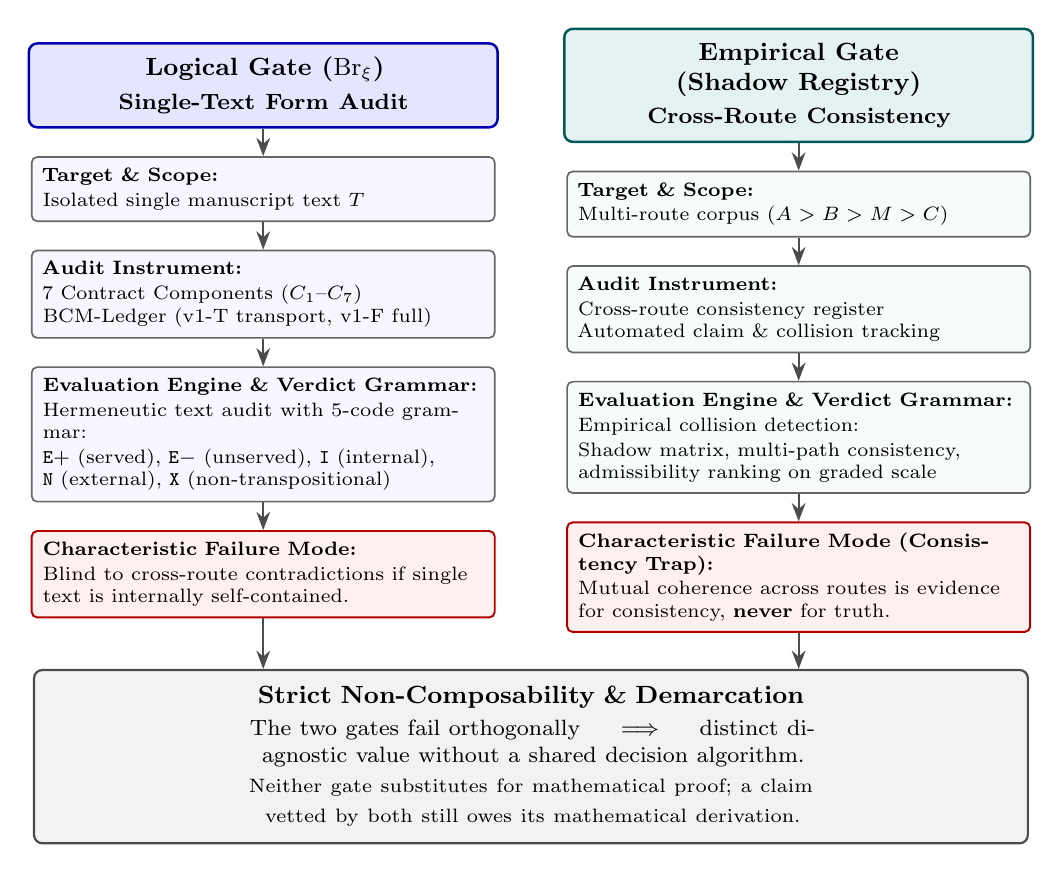
\begin{tikzpicture}[
  >=Stealth,
  node distance=0.6cm and 0.8cm,
  header/.style={draw=black!80, rounded corners=3pt, line width=0.9pt, align=center, font=\small\bfseries, inner sep=5pt},
  logcol/.style={header, fill=blue!10, draw=blue!70!black, text width=5.6cm},
  empcol/.style={header, fill=teal!10, draw=teal!70!black, text width=5.6cm},
  stepbox/.style={draw=black!60, rounded corners=2pt, line width=0.6pt, align=left, font=\scriptsize, inner sep=4pt, text width=5.6cm},
  alertbox/.style={draw=red!70!black, rounded corners=2pt, line width=0.7pt, fill=red!6, align=left, font=\scriptsize, inner sep=4pt, text width=5.6cm},
  barrier/.style={draw=black!70, rounded corners=3pt, line width=0.8pt, fill=gray!10, align=center, font=\small, inner sep=6pt, text width=12.2cm},
  arrow/.style={->, line width=0.8pt, draw=black!70}
]

  % Headers
  \node[logcol] (h1) at (0, 6.0) {Logical Gate ($\mathrm{Br}_\xi$)\\[1pt]\footnotesize Single-Text Form Audit};
  \node[empcol] (h2) at (6.8, 6.0) {Empirical Gate (Shadow Registry)\\[1pt]\footnotesize Cross-Route Consistency};

  % Steps Gate 1
  \node[stepbox, fill=blue!3] (s1_1) [below=0.35cm of h1] {
    \textbf{Target \& Scope:}\\[1pt]
    Isolated single manuscript text $T$
  };
  \node[stepbox, fill=blue!3] (s1_2) [below=0.35cm of s1_1] {
    \textbf{Audit Instrument:}\\[1pt]
    7 Contract Components ($C_1$--$C_7$)\\
    BCM-Ledger (v1-T transport, v1-F full)
  };
  \node[stepbox, fill=blue!3] (s1_3) [below=0.35cm of s1_2] {
    \textbf{Evaluation Engine \& Verdict Grammar:}\\[1pt]
    Hermeneutic text audit with 5-code grammar:\\[1pt]
    $\mathtt{E+}$ (served), $\mathtt{E-}$ (unserved), $\mathtt{I}$ (internal),\\
    $\mathtt{N}$ (external), $\mathtt{X}$ (non-transpositional)
  };
  \node[alertbox] (a1) [below=0.35cm of s1_3] {
    \textbf{Characteristic Failure Mode:}\\[1pt]
    Blind to cross-route contradictions if single text is internally self-contained.
  };

  % Steps Gate 2
  \node[stepbox, fill=teal!3] (s2_1) [below=0.35cm of h2] {
    \textbf{Target \& Scope:}\\[1pt]
    Multi-route corpus ($A > B > M > C$)
  };
  \node[stepbox, fill=teal!3] (s2_2) [below=0.35cm of s2_1] {
    \textbf{Audit Instrument:}\\[1pt]
    Cross-route consistency register\\
    Automated claim \& collision tracking
  };
  \node[stepbox, fill=teal!3] (s2_3) [below=0.35cm of s2_2] {
    \textbf{Evaluation Engine \& Verdict Grammar:}\\[1pt]
    Empirical collision detection:\\[1pt]
    Shadow matrix, multi-path consistency,\\
    admissibility ranking on graded scale
  };
  \node[alertbox] (a2) [below=0.35cm of s2_3] {
    \textbf{Characteristic Failure Mode (Consistency Trap):}\\[1pt]
    Mutual coherence across routes is evidence for consistency, \textbf{never} for truth.
  };

  % Connectors
  \draw[arrow] (h1) -- (s1_1);
  \draw[arrow] (s1_1) -- (s1_2);
  \draw[arrow] (s1_2) -- (s1_3);
  \draw[arrow] (s1_3) -- (a1);

  \draw[arrow] (h2) -- (s2_1);
  \draw[arrow] (s2_1) -- (s2_2);
  \draw[arrow] (s2_2) -- (s2_3);
  \draw[arrow] (s2_3) -- (a2);

  % Bottom Barrier
  \node[fit=(a1)(a2), inner sep=0pt] (failurepair) {};
  \node[barrier, anchor=north] (bar) at ($(failurepair.south)+(0,-0.45)$) {
    \textbf{Strict Non-Composability \& Demarcation}\\[2pt]
    \footnotesize The two gates fail orthogonally $\implies$ distinct diagnostic value without a shared decision algorithm.\\
    \scriptsize Neither gate substitutes for mathematical proof; a claim vetted by both still owes its mathematical derivation.
  };

  \draw[arrow] (a1.south) -- (a1.south |- bar.north);
  \draw[arrow] (a2.south) -- (a2.south |- bar.north);

\end{tikzpicture}%
}
\caption{Dual-gate proof assurance architecture: Logical Gate ($\mathrm{Br}_\xi$) vs.\ Empirical Gate (Shadow Registry).}
\label{fig:dual_gate_architecture}
\end{figure}

\begin{table}[htbp]
\centering
\footnotesize
\renewcommand{\arraystretch}{0.95}
\caption{Taxonomy of proof assurance and auditing gates in advanced mathematics.}
\label{tab:gate_taxonomy}\label{tab:tor_taxonomie}
\begin{tabularx}{\textwidth}{@{} >{\raggedright\arraybackslash}p{0.17\textwidth} >{\raggedright\arraybackslash}p{0.21\textwidth} >{\raggedright\arraybackslash}p{0.17\textwidth} >{\raggedright\arraybackslash}p{0.17\textwidth} >{\raggedright\arraybackslash}X@{}}
\toprule
Gate / Paradigm & Scope of Audit & Verifier / Trust Base & Output Format & Diagnostic Strength / Limit \\
\midrule
Logical Gate ($\mathrm{Br}_\xi$ / BCM) & Single transport step in mathematical text & Hermeneutic / domain expert & 5-code contract ledger (\texttt{E+}, \texttt{E-}, \texttt{I}, \texttt{N}, \texttt{X}) & Localizes exact unserved clause; judges form, not truth. \\
\addlinespace[4pt]
Empirical Gate (Shadow Registry) & Cross-route claim consistency across corpus & Automated registry lookup ($A>B>M>C$) & Consistency / collision matrix & Detects cross-text contradictions; subject to consistency trap. \\
\addlinespace[4pt]
Machine Formalization (Lean / Coq) & Deductive kernel across complete proof & Mechanized proof assistant & Binary validity certificate & Absolute deductive certainty; high formalization cost. \\
\addlinespace[4pt]
Certifying Algorithms (PCC / Runtime) & Algorithmic input-output pair & Algorithmic witness verifier & Com\-pu\-ta\-tion\-al cer\-tif\-i\-cate & Decidable instance checking; requires pre-agreed policy. \\
\bottomrule
\end{tabularx}
\end{table}

%=====================================================================
\section{A Protocol-Frozen Retrospective Two-Case Illustration
(v1-T)}\label{sec:calibration}

We illustrate the frozen v1-T instrument retrospectively on two historically
decided cases: a \emph{retrospective known-gap case}, a proof attempt whose
gap was later confirmed by its author, and an \emph{accepted control}, an
accepted proof with a structurally comparable transport step. The protocol ---
row set, five-code handbook, confidence scheme, independent second coding with
an explicit dissent rule, hindsight controls, and the success and falsification
criteria --- was written down and frozen before any source was read; the audits
changed none of it.

That temporal priority is documented internally, not externally. The protocol
was not publicly registered before coding; its temporal priority is documented
by the dated internal project record and the audit notes. We therefore use
``protocol-frozen'', not ``externally preregistered''. Where this paper says a
choice was fixed in advance, it means: prospectively frozen in the project
record before the two source-coding passes. A checksum computed today would
establish the identity of the file published today, not the date on which it
was frozen.

\subsection{Design and Instrument Version}

The two historical cases were coded with \textbf{BCM-Ledger v1-T}, the six-row
transport instrument frozen on 15 August 2026 before source coding. Its
version-scoped rows are T-R2a, T-R2b, T-R4a, T-R4b, T-R6, and T-R8, with the
case-neutral semantics reproduced in the table below. This is not the full v1-F
ledger of Section~\ref{sec:ledger}; the two versions are related only by the
published crosswalk (Section~\ref{sec:crosswalk}).

\begin{table}[htbp]
\centering
\small
\caption{The frozen six-row transport instrument (BCM-Ledger v1-T) and case-neutral test questions.}
\label{tab:frozen_instrument_v1t}
\begin{tabularx}{\textwidth}{@{}l X@{}}
\toprule
v1-T row & Case-neutral question of the frozen instrument \\
\midrule
T-R2a & Is the transport or transfer law written out explicitly, as a formula
        or statement with an address? \\
\addlinespace[3pt]
T-R2b & Are the transported quantities carried with a visible conversion
        factor? \\
\addlinespace[3pt]
T-R4a & Is the compensation or normalization mechanism named and located? \\
\addlinespace[3pt]
T-R4b & Is its existence and well-definedness proven in the text, not merely
        asserted? \\
\addlinespace[3pt]
T-R6 & Are second modes or case distinctions displayed and treated
       symmetrically? \\
\addlinespace[3pt]
T-R8 & Is the chain-closing compatibility derived rather than posited, and at
       which level (local or globally summed)? \\
\bottomrule
\end{tabularx}
\end{table}

The audited unit in each case is the central transport step, instantiated over
these six rows. Each row receives exactly one of the five codes of
Section~\ref{sec:ledger}. Each case was coded twice: a first audit and an
independent second coding whose auditor received only the frozen protocol and
the source, not the first coding. Success was fixed in advance: in the
known-gap case, at least one row must fire ($E{-}$/$N$) \emph{and} its address
must match the historically documented gap; in the control, no row may fire (an
$I$ is non-critical). Failure modes were fixed symmetrically: no firing, firing
at the wrong address, or a firing in the control.

\subsection{The Retrospective Known-Gap Case: The 1993 Fermat Announcement}

The first case is Wiles' 1993 proof announcement, audited through the
contemporaneous technical report of Rubin and
Silverberg~\cite{rubinsilverberg}; the audit therefore concerns the 1993
state of the argument \emph{as reported}, a scope limitation carried
explicitly. Both coders, independently, produced the same picture: the
transport law and its conversion quantities are explicit
($\text{T-R2a}, \text{T-R2b} = E{+}$), the compensating mechanism --- the Euler
system --- is named and located ($\text{T-R4a} = E{+}$), the case distinctions
are displayed ($\text{T-R6} = E{+}$), and exactly one row fires concordantly:
\emph{the existence of the named mechanism} ($\text{T-R4b} = E{-}$), at the
passage where the report states that the construction of a suitable Euler
system was ``not yet complete.'' The chain-closing row T-R8 was coded $E{-}$ by
the first coder (as a consequence of T-R4b) and $I$ by the second; under the
double-coding rule below the dissent is verdict-neutral, since the success
criterion was already met by T-R4b alone.

The address of the firing row is the passage that the report itself marks as
incomplete, and it is the obligation that the subsequent repair of the argument
had to discharge; the surrounding chain was not at issue there. The diagnostic
content lies as much in the four rows that did \emph{not} fire: the located gap
is narrow, not diffuse.
% TODO(operator, P2-7): the sentence above is deliberately anchored only to
% rubinsilverberg, which reports the 1993 state and the announced
% incompleteness but cannot document the 1994--95 repair. If a stronger claim
% about that repair is wanted in the version of record, add a primary or
% contemporaneous anchor for it (candidate to verify: Taylor--Wiles and Wiles,
% Ann. of Math. 141 (1995)) and cite it here. Do NOT strengthen the sentence
% without such an anchor.

\subsection{The Accepted Control: An Accepted Transport Step}

The second case is Prasad's volume formula~\cite{prasad}, whose
local-to-global normalization step is an accepted instance of the same
transport shape. Both coders found no firing row: five rows explicitly
discharged in both codings; one row (T-R6) split between $I$ (first coder,
on account of the author-declared function-field asymmetry: the relevant
convergence statement is proved over number fields by an external
reference, while for global function fields the text records only that ``a
similar proof applies'' (\cite{prasad}, \S3.2)) and $E{+}$
(second coder), which is verdict-neutral because $I$ is non-critical by the
frozen protocol. The scope reservation admitted by the protocol --- an audit of
a transport step inside an accepted proof rather than of the whole paper --- did
not have to be invoked as an $X$. The control also supplies a positive image of
what the rows measure: the normalization constant is carried as a visible factor
rather than silently set to one, and the chain closes through an addressed
chain of equations rather than an assertion that it ``follows formally.''
This is the only accepted control in this paper.

\subsection{The Complete Code Matrix}\label{sec:matrix}

Both codings of both cases are reported in full in Table~\ref{tab:code_matrix_retrospective}. Columns F1 and F2 are the
first audit and the independent second coding of the known-gap case (Wiles
1993, as reported); columns P1 and P2 are the first audit and the independent
second coding of the accepted control (Prasad). No cell below is a consensus
value.

\begin{table}[htbp]
\centering
\small
\setlength{\tabcolsep}{3.5pt}
\caption{Complete double-coded audit matrix for the retrospective test cases (Wiles 1993 vs.\ Prasad 1989).}
\label{tab:code_matrix_retrospective}
\begin{tabular}{@{}lcccc@{}}
\toprule
v1-T row & F1 (Wiles 1st) & F2 (Wiles 2nd) & P1 (Prasad 1st) & P2 (Prasad 2nd) \\
\midrule
T-R2a & $E{+}$ & $E{+}$ & $E{+}$ & $E{+}$ \\
\addlinespace[3pt]
T-R2b & $E{+}$ & $E{+}$ & $E{+}$ & $E{+}$ \\
\addlinespace[3pt]
T-R4a & $E{+}$ & $E{+}$ & $E{+}$ & $E{+}$ \\
\addlinespace[3pt]
T-R4b & $E{-}$ & $E{-}$ & $E{+}$ & $E{+}$ \\
\addlinespace[3pt]
T-R6 & $E{+}$ & $E{+}$ & $I$ & $E{+}$ \\
\addlinespace[3pt]
T-R8 & $E{-}$ & $I$ & $E{+}$ & $E{+}$ \\
\bottomrule
\end{tabular}
\end{table}

\noindent
Inter-coder concordance was 10 of 12 case-row comparisons. The two dissents are
F/T-R8 and P/T-R6; neither was harmonized. The rule under which these codings
were read is the following.

\begin{quote}
A critical firing in the known-gap case counts toward the pre-specified success
criterion only when both coders assign $E{-}$/$N$ to the same row. A control
failure is recorded if either coder assigns $E{-}$/$N$. Discordant code pairs
remain visible and are never replaced by a synthetic consensus code.
\end{quote}

\noindent
Under this rule exactly one row counts as a concordant critical firing in the
known-gap case, namely T-R4b; in the control no coding contains $E{-}$ or $N$
at all. Stating the rule explicitly is a disclosure of the rule already
applied, not a retrospective change to the codings.

\subsection{Anchoring and Availability}\label{sec:anchors}

Every coding in both audits carries a verbatim quotation with a page or section
anchor from the named edition, together with the three-axis confidence record
prescribed by the frozen protocol: source binding, criterion fit, and substance
status, each on a three-point scale. Those per-row anchor tables live in the
dated project record --- the frozen protocol, four audit notes (a first audit
and an independent second coding for each case), and the operator synthesis
that carries the verdict wording. This draft reproduces the complete code
matrix but not the per-row anchors.
% TODO(operator, P1-5): before upload, release the per-row anchor tables (row,
% version/edition, page or section, short quotation, both raw codes, three-axis
% confidence) as a citable supplement and reference it here. Internal file names
% without accessible content do not satisfy this obligation for a public
% version. Note the pipeline rule that _proof-notes/ is private by default: the
% staged release of individual closed notes needs an explicit operator decision.

\subsection{\texorpdfstring{What the Illustration Shows---And What It Does Not}{What the Illustration Shows -- And What It Does Not}}

Under the pre-specified criteria, the two pre-specified case criteria were met
in this illustration: the confirmed gap of the 1993 argument is located at a
single concordantly firing row whose address matches the historically
documented gap, and neither coding assigned $E{-}$ or $N$ in this one control
case. We state the outcome in the formulation fixed in the protocol: the two
cases are \emph{consistent with the certificate's design intent}. They are one
retrospective known-gap case and one accepted control --- an illustration, not
a validation statistic, and not a measurement of any rate. The exercise is a
retrodiction, not a prediction: the historical outcome was known to both
coders, and its value rests entirely on the row assignment having been fixed in
writing before reading, with the falsifiable alternatives (wrong address,
diffuse firing, a firing in the control) stated in advance and not realized.

Two further limits belong here. The illustration concerns v1-T only; it does
not exercise the full v1-F ledger of Section~\ref{sec:ledger}, and nothing
below inherits support from it. And with two cases and two coders, the reported
concordance describes this pair of audits; it is not an estimate of the
instrument's reliability.

%=====================================================================
\section{The abc Instantiation}\label{sec:abc}

\subsection{The Gate Case}\label{sec:abc-gate}

This section reports the one instantiation contained in this paper. It is a
\emph{selected-rows} instantiation carried out with rows of
\textbf{BCM-Ledger v1-F} (Section~\ref{sec:ledger}): the rows exercised
below are F-R2a, F-R2b, F-R4a, F-R4b, F-R6a, F-R6b and, where its trigger
fires, F-R8; the remaining rows (F-R0, F-R1, F-R3, F-R5, F-R7) are not
coded here, and a coding of the complete matrix for these cases is deferred
to a later version. The row labels below carry the prefix \texttt{F-}, and
none of them is the row of the same number in the frozen transport ledger
v1-T used in Section~\ref{sec:calibration}.

The step at issue is a substep in the proof of Corollary~3.12 in the third
volume of inter-universal Teichmüller theory~\cite{Mochizuki2021c}. Its
conclusion has the form axiomatized in Definition~\ref{def:bridge}: a
log-volumetric reading $\nu_q(x)$ of the $q$-pilot object $x \in X_q$ is
asserted to lie in a target region $H_\Theta = \mathbb{R}_{\le -|\log\Theta|}$
fixed on the $\Theta$-side, where the two sides share no common evaluation by
construction. The step labeled (xi-e)$\to$(xi-f) is where that membership is
drawn.

That this step carries the load is the result of Part~1~\cite{part1} and is
taken as given. The criterion asks a different question of the same passage:
not where the argument is thin, but which contract components the presentation
serves. Everything below is read in the register of Section~\ref{sec:scope} ---
a row that does not deliver names a clause a complete argument must supply, and
says nothing about whether it can be supplied.

\subsection{The Audited Substep of the Original Argument}\label{sec:abc-original}

The audit covers the rows activated at the substep itself: F-R2a, F-R2b, F-R4a,
F-R4b, F-R6a, F-R6b and, by the multi-mode trigger, F-R8. The remaining rows of
the ledger carry no verdict here. The table below collects the verdicts; what
follows are the grounds.

At the audited substep no intra-link transport operation is performed; F-R2a is
therefore X at that substep, not E+. The cross-framework numerical
identification needed by the conclusion is assessed separately under F-R2b and
F-R6a. A common evaluation in C does not discharge Component 6 unless the
required compatibility identities are present and addressed. What supports the
first of these statements is that the parallel-transport mechanism is described
as one that ``does not consist of a simple instance of transport of some
set-theoretic region'', and that the $q$-side readout is declared
``coric''/``fixed'' and expressly not subject to the indeterminacies the
$\Theta$-side carries: the readout keeps its identity by stipulation and by the
absence of a transport step, not by a proved relation.

F-R2b partially delivers, and no more than that. At (xi-d) the two sides are
brought into one evaluation, only thereby yielding what the text calls
``completely comparable objects'', and global arithmetic degrees are read as
log-volumes on both sides. That is an identification carried by a shared reading
convention rather than by a visible conversion factor or a compatibility
equation, and the crosswalk caps a row of that shape at \texttt{I}. The row
reaches that ceiling rather than falling below it because the identification is
itself exhibited at a named substep and can be read off the text: what the
documented reconstruction lacks is a derivation of the identification, not the
identification. At this step the row is moreover not separable from F-R6a, the
identification of the two evaluation containers being part of the bridge step
itself.

F-R6a does not deliver. A numerical evaluation $\nu_C$ on the container is
exhibited; what the hardened Component~6 requires in addition --- the
compatibility identities the claim needs, in particular $\nu_C \circ i_q = \nu_q$ on the
stated source domain --- is not derived at the audited step. The
source-side reading is held fixed by stipulation --- the passage quoted under
F-R2a above, which declares the readout ``coric''/``fixed'' and exempt from the
$\Theta$-side indeterminacies --- and a stipulated invariance is
not the identity Component~6 asks for. The row would deliver partially only if a
documented reconstruction of that identity were supplied; this audit supplies
none. The earlier reading of this passage, which recorded Component~6 as served,
rested on the weaker either/or formulation that Definition~\ref{def:bridge} no
longer contains.

F-R6b does not deliver, and it is the principal chain-closing obligation. The
membership is not derived from the admissible linkage but
obtained from a condition imposed on the admissible operations: the inclusion
``then follows formally'' from the requirement that the construction of the
output possibilities constitutes, in particular, a construction of the input
readout, and a summary of the same argument speaks of ``two tautologically
equivalent ways'' to compute one log-volume. Where the named order lemma of
Component~7 would stand --- with its hypotheses, a claim of applicability at
this step, and a proof address --- a pair of declared properties of the
algorithm's output stands instead. The row records the absence of such an
addressed lemma. It does not record a judgment on whether one could be proved.

Two fairness statements belong to that verdict rather than beside it. Confidence
is high precisely because the load-bearing passages use those words themselves;
and ``tautological'' is used affirmatively there, the text elsewhere calling its
conclusions nontrivial albeit essentially tautological. For that author the
tautologicity is the point, not an admission, and reading it as self-refutation
would be an authority argument in reverse.

The load rows require the second split. In the audited volume the load carried
by the theta values $q^{j^2}$ is named but not quantified --- what is booked at
the identified site are labels rather than magnitude --- and at the bridge step
the internal structure is deliberately set aside. The quantification is not
omitted but declared, its address given as the explicit log-volume computation
in \S1 of the fourth volume~\cite{Mochizuki2021d}, and that address pays out:
the load is carried through that computation to the closed form $(\ell+1)/24$
and stands in the final bound as
$-\tfrac{1}{6}\bigl(1-12/\ell^{2}\bigr)\log q$. F-R4a therefore delivers for the
composite of the two volumes; F-R4b does not, that section taking the
corollary's conclusion as an input and quantifying downstream of the bridge.
Both rows are reported at Component~5, which is where the crosswalk localizes
the load budget. An early concern recorded in the ledger note of May 2026, that
the $j^2$ factors might vanish in one coordinate and return unbooked, does not
hold for the composite and is withdrawn: booked elsewhere as announced is not
the same finding as unbooked.

F-R8 is triggered here, since the claim's domain model contains an alternative
mode that bears on the order relation. It partially delivers: the second mode is
named, the vertical-shift conflict stated and its price declared, but it is
converted beforehand into a one-sided inequality and suspended at the step
itself.

The audited rows therefore do not reduce to a single surviving obligation.
F-R2a is out of scope at the substep, F-R2b partially delivers, and F-R4a
delivers for the composite of the two volumes. Against that profile the
remaining obligations are weighted as follows. The audit distinguishes one
principal chain-closing obligation from three additional findings: F-R6b is the
principal order-lemma obligation; F-R6a records the missing compatibility
identity of the common evaluation; F-R4b records a separate
booking-at-the-bridge deficit; and triggered F-R8 records partial treatment of
the second mode. The ledger therefore localizes differently weighted findings
rather than a single surviving row.

\subsection{A Comparative Discrimination Case: Joshi's ATS
Program}\label{sec:abc-control}

A criterion that returns the same verdict everywhere is a template, not an
instrument. We therefore apply the same selected v1-F rows, with unchanged
row semantics, to a second program of the same dispute complex reaching
the same inequality by other means: Joshi's arithmetic Teichmüller
spaces~\cite{JoshiATSIII,JoshiATSIV}. This case is not a positive control and
supplies no independent confirmation of the inequality. It is a methodologically
distinct, preliminary comparison used to ask whether the same selected rows
produce a different pattern of served, reconstructed, and unserved obligations.
The only accepted control in this paper is the one in
Section~\ref{sec:calibration}. It does: the profile differs, and the remaining
obligation has a different address and a different shape.

F-R2a rests on a proved relation rather than a stipulation: the scaling relation
between the valuations along the program's own link is a theorem there, and the
$j^2$ factor is carried visibly into an explicitly defined log-volumetric scale.
Here the split separates cleanly, which is why this audit produced it. F-R2b, by
contrast, rests on the choice of the same global normalization on both sides ---
a convention, not an exhibited conversion factor --- and therefore partially
delivers at most, exactly as the crosswalk caps a row of that shape. It reaches
that ceiling because the normalization is explicitly chosen and stated, so the
reconstruction is documented; what is absent is a conversion factor carried
visibly through the step.

The load obligation was audited before the split was introduced and is
therefore reported as a single verdict, at F-R4a. The load is booked against a
global constraint, the product formula, with high confidence for the address
and medium for completeness, the compensating renormalization being inferred
rather than constructed. The address is served and completeness is not
established, so the row delivers for the address and only partially for
completeness --- not unqualifiedly. An audit at the split would have to
separate the served address from the inferred existence; this one did not, and
F-R4b therefore carries no separate finding in this case.

F-R8 is delivered as the row asks: a global Frobenius shift is named, deployed
asymmetrically for the two bounds, and flagged by the author as a correction to
his own earlier version --- and because it is visible, the remaining obligation
has an address at all.

F-R6a partially delivers, and the shape of the remainder is this case's yield.
The order relation carrying the conclusion holds between sums over all places;
place-wise it is expressly disclaimed, the author stating that local
term-by-term comparisons at each prime cannot be made without violating the
concurrent normalizations, and the theorem's own remark holding that this choice
``precludes direct comparison of various local quantities''. The identification
of the two evaluations rests on identical global normalization and is called a
tautology at that point. That word must be scoped: it occurs at several places in
the program with different reach, only its use for the middle equality of the
carrying theorem is load-bearing here, and it is not the author calling his own
arithmetic proof of the corollary a tautology.

F-R6b is where this case differs most sharply in form from the original
argument, and where the auditor's boundary must be observed most carefully. What
the row tests is present: a named theorem with stated hypotheses, an assertion of
its applicability at the step, and a written-out proof with an address. That is
the whole of what a served F-R6b certifies. Against it stands a substance
finding, reported here at F-R6b because that is where the obligation it concerns
is localized: the substance audit of Part~5~\cite{part5} typed the core step of
that proof as open against the construction it cites, so the core of the
obligation remains open. That finding is not a form verdict, and the auditor
does not adjudicate it.

Two corrections revised the historical reading of this case in opposite
directions. Within the particular normalization framework named in the
audited Part~4~\cite{part4}, the identification was read as definitional
rather than a concealed choice; this is not an unconditional identification
across ATS fields, place ranges or volume constructions. Set stability and
the pinning of the measure remain separate obligations. The Part~5 substance
finding~\cite{part5} is distinct from that form reading. The rigidity result
cited in the historical discussion~\cite{part6} is conditional on its stated
field, all-place and normalization hypotheses; it removes no such hypotheses
and supplies no unconditional ATS or volume conclusion.
Table~\ref{tab:abc_ats_comparison} retains the historical comparative audit
results, scoped to the versions audited. The volume carrying the abc
conclusion describes itself as a preliminary version for comments.

\begin{table}[htbp]
\centering
\small
\caption{Comparative audit profile for the abc transport step (original IUT presentation vs.\ ATS program).}
\label{tab:abc_ats_comparison}
\begin{tabularx}{\textwidth}{@{}l X X@{}}
\toprule
v1-F row & Original argument & Comparative case (ATS program) \\
\midrule
F-R2a & out of scope (X): no intra-link transport operation at the substep
   & delivers (high): a proved scaling relation along the program's own
     link \\
F-R2b & partially delivers: identification by a shared reading convention;
     not separable from F-R6a here
   & partially delivers: the same global normalization, set by convention \\
F-R4a & delivers (high) for the composite of the two volumes
   & audited unsplit, reported here: delivers for the address, partial for
     completeness --- the compensating renormalization is inferred rather than
     constructed \\
F-R4b & does not deliver (high): quantified downstream of the bridge
   & no separate finding: not audited at the split (see F-R4a) \\
F-R6a & does not deliver: no compatibility identity derived at the step
   & partially delivers (high): order after summation, place-wise
     disclaimed \\
F-R6b & does not deliver (high): membership ``follows formally''
   & textually served: named theorem, hypotheses, proof address; core step
     typed as open by a substance audit \\
F-R8 & partially delivers (high): named and priced, suspended at the step
   & delivers (high): named, asymmetric, declared \\
\bottomrule
\end{tabularx}
\end{table}

\noindent
The audited unit was these rows at the identified step in both cases; the
remaining rows of Section~\ref{sec:ledger} carry no verdict here, and a row
coded X is not counted against either presentation. What the comparison
localizes is a difference in the \emph{form} of the remaining obligation: a pair
of declared properties distributed over a remark and several substeps, against a
single named equality with a written-out proof. Whether that proof is correct is
not a question this instrument answers.

\subsection{Inheritance: What Travels with a Citation}\label{sec:abc-inheritance}

A downstream inheritance example moves the question past the audited step. Two
application papers by
Zhou~\cite{ZhouI,ZhouII} derive Diophantine consequences resting on the
inequality of Corollary~3.12, and the audit asked one question: how the bridge is
taken over. In the first it appears as a proposition whose entire proof is one
sentence --- ``The proposition follows from the $\mu_6$-version of [37],
Corollary~3.12'', the reference being to the third volume in that paper's
numbering --- and is used exactly once, after which the downstream chain
proceeds. In the second, in the version audited, the corollary is not named at
all: the bridge is inherited through the first paper and extended to a new class
of initial data by tracking a single hypothesis through the cited volumes,
without the bridge step being touched. What both papers contribute of their own
lies on the far side of the bridge.

None of this is irregular: citing an established result instead of re-deriving it
is what citation is for. What makes the structural point visible is that both
papers state plainly where they omit a step of their own. Those reservations
attach to their own omissions and none attaches to the imported step --- not
because the authors declined to make one, but because nothing in a citation
carries a contract state. A served row and an unserved row travel identically
through a bibliography.

This is the practical case for a contract certificate as a \emph{citation
interface}. An audited ledger is a citable artifact: it states, row by row, what
the cited result was found to serve and what it was found to leave open, so that
an importing paper inherits a known contract state instead of an unknown one.
Under such a discipline --- formulated in Part~3~\cite{part3} as an import ledger
--- neither paper's mathematics would change; each would carry one further line
naming the row its import leaves unserved. Both findings are scoped to the
versions audited, the second paper describing itself as an older version to be
updated, and one question the audit left open --- whether a normalizing factor in
the first paper's statement renormalizes the same quantity the corollary carries
--- is left open here.

\subsection{An External Point of Comparison}\label{sec:abc-external}

The last item in this section is not ours. An interim report of a formalization
project, published in July 2026~\cite{LANA2026}, isolates a compatibility problem
at the same passage --- and isolates it in the shape of a contract. Its
condition, numbered (9-1) there, requires the existence of a suitable choice of
integral structure under which two evaluation isomorphisms with a common target
agree: one arising from the $q$-pilot in its native structure, the other obtained
anabelian and Kummer-theoretically and subject to indeterminacies. The report
states that the project ``has not yet reconstructed a proof of the required
compatibility'', and that the proof of the final numerical inequality ``hinges on
the compatibility (9-1) which is not manifestly false. However, we, the LANA
project, do not have a proof of (9-1) at this time.''

Read against Definition~\ref{def:bridge}, the proposed correspondence is
object-wise, not a verified transfer: a common target quotient, typed maps,
readouts, integral structures and indeterminacies would have to be identified
with their actual objects, domains, quantifiers and implication direction.
The existence of a quotient or a shared target alone does not serve the
compatibility identities of Component~6. If an equality of readouts has been
established in the common value space $V$, reflexivity gives the numerical
comparison in $V$, not conversely. This does not by itself give the container
order (H2): $\nu_C$ need not reflect order. Equality of the identified images
in $C$ gives (H2) by reflexivity in $C$; numerical comparison alone requires
order reflection or a separately addressed proof of (H2). Membership in
$H_\Theta$ additionally requires the applicable (H1)--(H5), including the
target bound (H5). No such IUT-to-C7 bridge is proved by this comparison.

The ledger note that fixed the criterion in May 2026 recorded a conditional
expectation: should a formalization effort carry this passage, the contract would
have to appear in it as a lemma. The report has that shape. In this single
interim report, at this single passage, an independently formulated
compatibility condition occupies a position analogous to F-R6b. We record a
\textit{post hoc} structural resemblance, not convergence on the general criterion and
not confirmation of our case verdict. No claim of precedence is made either; the
analysis is that project's own and in its own terms.
The limits are equally plain: the document is an interim report without a final
verdict and records internal dissent, and our mapping is object-wise, not a proof
that (9-1) and component~7 are equivalent. The report's own position ---
required, unproven, not manifestly false --- is precisely what the verdict
grammar of Section~\ref{sec:ledger} exists to express: a row that does not
deliver localizes a burden and refutes nothing.

%=====================================================================
\section{Outlook: RH Uniformity Claims}\label{sec:rh}

The criterion is not specific to the abc literature. Positivity approaches
to the Riemann Hypothesis contain the same two shapes --- transport steps
(finite-model results carried to a limit object) and global-only claims
(positivity available only after summation) --- and the corresponding
ledger rows could be instantiated there: uniformity obligations for
finite-section bounds, quotient obligations where majorization arguments
are excluded, and an explicit payment obligation for archimedean mass. We
defer any such instantiation to a dedicated treatment, synchronized with the
self-application part of this series, because our own program is among
the audited objects there and the protocol-freezing discipline of
Section~\ref{sec:calibration} requires the operationalized rows, primary
sources, and claim boundaries to be fixed before the section is written.
This section is an outlook and not an instantiation: the present paper
deliberately contains no RH-side verdicts.

%=====================================================================
\section{A Related Structure: Global-Only Claims}\label{sec:global}

A recurring shape in both instantiation domains is the \emph{global-only}
claim: a statement asserted to hold only after summation over all places,
with local, place-wise access explicitly unavailable. In Weil-positivity
approaches to RH the positivity of a quadratic form is a global sum whose
individual terms carry no sign; in the abc literature, the source of the
principal repair program restricts its comparisons to the summed level in
so many words (``one cannot make local term by term comparisons at each
prime''~\cite{JoshiATSIII,JoshiATSIV}), and its normalization mechanism is a
product-formula constraint --- again a statement about a product over all
places, not about any single factor. The audit trail for both readings is in
Parts 4 and 5 of this series~\cite{part4,part5}.
% TODO(operator, P2-7): the quotation above is now anchored to the primary ATS
% source rather than to our own audit parts, but it still lacks a precise
% locator. Add the volume, section or page of ATS III/IV for this sentence
% before upload; the same locator is also wanted at the parallel passage in
% Section \ref{sec:abc-control}.

For the criterion this shape triggers a specific obligation. Where a claim
lives only at the summed level, the contract components 6--7 cannot be
served place-wise; what must then be supplied is a \emph{contract lemma}. We
state what such a lemma has to contain.

\begin{definition}[Global-only contract lemma]\label{def:globallemma}
Let $(x_v)_{v\in\Sigma}$ be an admissible family, let $G((x_v)_v)=e$ be a
stated global constraint, and let $S((x_v)_v)$ be the aggregate used by the
claim. A global-only contract lemma is a named, addressed statement that
specifies (G1) the admissible class and convergence/domain conditions, (G2)
the exact global constraint, (G3) the aggregate equality or order implication
needed for the claim, and (G4) the local degrees of freedom that remain after
imposing the constraint. It discharges F-R6b only at the global level. A
place-wise rigidity conclusion requires an additional named injectivity,
strictness, or uniqueness hypothesis and may not be inferred from globality
alone.
\end{definition}

In this paper the definition is an outlook interface, not a second
instantiation; no global-only ledger verdict is reported. The tool supplement
of this series~\cite{gnc} carries out a construction of this kind for the
global normalization of the abc repair program, and the rigidity theorem of
Part 6~\cite{part6} exhibits one case in which a global multiplicative
constraint over all places, together with the hypotheses stated there, does
force place-wise rigidity --- which is an instance of (G4) discharged under
named additional hypotheses, not a general license to read rigidity off
globality. Within v1-F the triggered row F-R8 is activated at the global level
only when several global modes or branches can affect the order of the
aggregate. The lesson for auditing is symmetrical: global-only is not a defect,
but it converts local obligations into a single named global one --- and the
audit must check that this one is discharged, not dissolved into notation.

\subsection{Current Developments in Parts 4--6}\label{sec:current-series}

The later v0.3 papers are additional, version-specific research references,
not replacements for the v0.2 pins used in the retrospective audit above.
Part~4~\cite{part4current} retains a partially documented normalization
convention while separating the typed log-image, hull and log-volume
contracts. Part~5~\cite{part5current} distinguishes raw and normalized
coordinates and requires the actual common fixed coordinates, coefficient
transformation and period-image action for its Frobenius route. It also
records the absolute-value bars actually printed in the narrowly checked
ATS-III corollary; the earlier atomic-sign exculpation is withdrawn under
the explicit Tate-place and finiteness assumptions there. These later
findings do not recode the historical rows or decide the whole ATS, abc or
IUT chain.

In the standard-modulus normalization of Part~6~\cite{part6current}, local
degree factors are included so that
\[
 \sum_{v\in M_L}\log b_v(x)=0\qquad(x\in L^\times).
\]
For one fixed number field $L$, all its places including the archimedean
ones, real weights independent of $x$, and every $x\in L^\times$,
writing the local norm realization as $\rho_v=b_v^{a_v}$, the
weighted product formula concerns the final effective weights
\[
 \beta_v=a_v\lambda_v,\qquad
 \sum_{v\in M_L}\beta_v\log b_v(x)=0\quad\text{for all }x\in L^\times.
\]
Under these hypotheses rigidity gives $\beta_v=c$; it does not identify
the raw $\lambda_v$ with $c$ when degree factors are separate. A constant
global factor, including $j^2$, is allowed. Tests restricted to $L^\times$
at places of an extension $L'$ do not determine the individual $L'$ weights.
Common field, norm and freeze identifications remain prerequisites for a
cross-branch comparison.

For a quantity consumer, the required family is linear:
\[
 Q_y=\sum_v\beta_{y,v}q_v,\qquad Q_{\rm ref}=\sum_v q_v,
 \qquad Q_y=c_yQ_{\rm ref},
\]
with $y$-independent $q_v$ and finite sums or justified absolute convergence.
The last equality is conditional on the same effective-weight hypotheses;
$Q_{\rm ref}=Q_{\rm cl}$ is an additional classical-reference bridge.
Pointwise normalization (5.3.3) yields the classical degree on $L^\times$
and height on $\mathbb P^n(L)$ under its stated identification, without an
automatic algebraic-extension or line-bundle-height transfer. Membership
and nonmembership of measures and log-volumes in this class remain unknown;
an arbitrary ATS hull is not silently identified with a maximal-order module
hull. These are current scope qualifications, not new F-R6 verdict codes.

%=====================================================================
\section{Limitations and Fairness}\label{sec:limits}

Four limitations bound everything above. \emph{First}, the criterion judges
form. No verdict in this paper or in the series is a truth verdict: not
about abc, not about IUT, not about any audited program. An unserved
ledger row is an obligation with an address; theorems are refuted by
mathematics, not by audits. What the auditor certifies is narrower still: that
an obligation is present, typed and addressable in a named version, never that
the mathematics it names is sound. \emph{Second}, the audit frame is neutral in
the underlying controversy. The same rows are applied to every audited text ---
the original program, its critics' reading, and the repair program ---
and the retrospective illustration of Section~\ref{sec:calibration} was
designed with a symmetric falsification criterion precisely so that the
instrument could have failed. \emph{Third}, the evidential basis is small by
construction and version-scoped: one retrospective known-gap case and one
accepted control under v1-T, one abc instantiation with one comparative
discrimination case under v1-F, plus a downstream inheritance example and an
external comparison. Nothing in the v1-F instantiation inherits support from
the v1-T illustration. We use the formulation fixed in the protocol,
``consistent with design intent'', and avoid ``validated'' throughout.
\emph{Fourth}, a fairness protocol governs the
practice: a verdict that depends on the audited author's own wording
carries that wording as a verbatim quotation with an address from a named
version; every other verdict argued in the running text is carried by a
paraphrase of the passage or feature relied on in the named version, or by
a citation into the published series part that documents it; the row-code
matrices are summaries
of archived audit records whose per-row anchor tables are not yet published
--- until the planned supplement appears, the matrices are to be read as
summaries of those records, not as independently checkable claims
(Section~\ref{sec:anchors}); confidence is stated in a fixed three-axis
scheme; findings
of the form ``the text does not show'' are never promoted to ``this is
false''; and audited authors' own scope statements are quoted, not
paraphrased, wherever a verdict depends on them.

The two retrospective cases also use different source genres and audited
versions: the Wiles case is accessed through the contemporaneous report by
Rubin--Silverberg, whereas the Prasad case uses the primary paper. Their
raw v1-T pairs remain visible: the Wiles T-R8 pair is $(E-,I)$ and the
Prasad T-R6 pair $(I,E+)$. This source asymmetry and the $10/12$ agreement
do not estimate reliability, discrimination or a false-alarm rate; neither
pair is silently converted into a v1-F F-R8 code. The LANA comparison still
requires its separate object, domain, quantifier and implication-direction
bridge; no equivalence or confirmation follows from structural resemblance.

%=====================================================================
\section{Conclusion}\label{sec:conclusion}

The current illustration now preserves the full conditional C7 contract;
the incomplete earlier diagram has been corrected without changing the
definition or the raw retrospective codes. Current Parts 4--6 refine the
remaining normalization and quantity-consumer obligations without supplying
a general methodological validation or closing the field, period, volume
or LANA transfer bridges.



We have stated a checkable form criterion for transport arguments: seven
contract components, a versioned ledger with a three-verdict grammar over five
raw codes, and an audit practice with verbatim anchoring and evaluation
criteria fixed before coding. Its position among existing structures is
specific --- the closest heuristic analogue is the certifying-algorithms
tradition, but the artifact here is reconstructed by a third-party auditor
rather than issued by the prover, and what a check establishes is textual
contract completeness rather than correctness --- and, within the bounded
corpus surveyed here, we found no work occupying the same place in the
mathematics-controversy literature.

The contribution established here is one abc instantiation of a form-audit
criterion. The two historical cases illustrate v1-T retrospectively; they do
not validate the full v1-F instrument. RH and global-only applications remain
future work. In the protocol-frozen two-case illustration, the pre-specified
criteria were met. Applied to the selected abc transport step, the ledger
replaces a diffuse disagreement about that step with a profile of named
obligations, weighted and each with a citation; it does not adjudicate the
controversy that surrounds it. What the criterion cannot do is prove anything,
and a served row certifies no mathematics. Its ambition is smaller and, we
believe, useful: that disagreements about transport claims can be conducted as
disagreements about named contract clauses --- checkable, quotable, and
revisable when the text changes.

%=====================================================================
% AI disclosure. The path is relative to the BUILD WORKING DIRECTORY, not to
% this file. Verified 2026-08-16 by compiling with cwd = paper/ , where it
% resolves to .RESEARCH/_templates/disclosure/ai_disclosure_STANDARD.tex and
% the disclosure is visible in the PDF. Compiling from any other directory
% requires adapting the path (or passing -include-directory).
% =============================================================================
% AI DISCLOSURE -- PIPELINE STANDARD, ENGLISH VERSION (since 2026-08-17, T-20260817-02)
% =============================================================================
% Language-pure version for English-only manuscripts. Text copied verbatim
% from the English block of ai_disclosure_STANDARD.tex (no content change) --
% only the heading is now language-pure and the German block is dropped. The
% bilingual file ai_disclosure_STANDARD.tex remains unchanged (existing
% references may keep pointing to it).
%
% DEVIATING DOWNWARD: If a paper genuinely used substantially less AI, do NOT
% switch to a different file -- weaken the wording here instead, e.g. replace
% "extensively in all phases" with the phases that actually applied, and
% strike whatever did not happen from the quality-assurance list. Principle:
% state honestly what happened -- do not hedge.
%
% Usage (English-only manuscripts only):
%   \input{../../_templates/disclosure/ai_disclosure_STANDARD_en}
% =============================================================================

\section*{AI Disclosure}

\noindent
AI systems were used extensively in all phases of this work: conception
and research discussion, literature and source work, mathematical analysis
and proof development, creation and checking of the computational scripts,
execution and evaluation of the computational runs, text, translation, and
typesetting.

\medskip

\noindent
Quality assurance: use of several independent models from different
providers with counter-checks and adversarial AI reviews; traceable,
versioned computational scripts with stored result files and checksums;
continuously maintained proof and register documents; strict claim hygiene
(assertions only with documented evidence, addenda instead of silent
corrections); changelogs across all versions.


%=====================================================================
\begin{thebibliography}{99}
\frenchspacing
\sloppy
\emergencystretch=3em
\hbadness=10000


\bibitem{Aberdein2023}
A.~Aberdein,
\emph{Deep Disagreement in Mathematics},
Global Philosophy \textbf{33} (2023), no.~1, article~17.
DOI: 10.1007/s10516-023-09653-7 (arXiv:2210.16488).

\bibitem{Andersen2017}
L.~E.~Andersen,
\emph{On the Nature and Role of Peer Review in Mathematics},
Accountability in Research \textbf{24} (2017), no.~3, 177--192.
DOI: 10.1080/08989621.2016.1274885.

\bibitem{Andersen2020}
L.~E.~Andersen,
\emph{Acceptable gaps in mathematical proofs},
Synthese \textbf{197} (2020), no.~1, 233--247.
DOI: 10.1007/s11229-018-1778-8.

\bibitem{GSN2021}
Assurance Case Working Group (ACWG),
\emph{Goal Structuring Notation Community Standard (Version 3)},
Safety-Critical Systems Club (SCSC), 4 May 2021.
Available at \url{https://scsc.uk/r1386.pdf}.

\bibitem{Avigad2021}
J.~Avigad,
\emph{Reliability of mathematical inference},
Synthese \textbf{198} (2021), no.~8, 7377--7399.
DOI: 10.1007/s11229-019-02524-y.

\bibitem{Bloomfield2021}
R.~Bloomfield and J.~Rushby,
\emph{Assurance 2.0: A Manifesto},
arXiv:2004.10474v3 [cs.SE], 2020 (revised 14 January 2021).
DOI: 10.48550/arXiv.2004.10474.

\bibitem{Blum1995}
M.~Blum and S.~Kannan,
\emph{Designing programs that check their work},
Journal of the ACM \textbf{42} (1995), no.~1, 269--291.
DOI: 10.1145/200836.200880.

\bibitem{Buzzard2020}
K.~Buzzard, J.~Commelin and P.~Massot,
\emph{Formalising perfectoid spaces},
in: Proceedings of the 9th ACM SIGPLAN International Conference on
Certified Programs and Proofs (CPP 2020), ACM, 2020, 299--312.
DOI: 10.1145/3372885.3373830.

\bibitem{Castelvecchi2020}
D.~Castelvecchi,
\emph{Mathematical proof that rocked number theory will be published},
Nature \textbf{580} (2020), no.~7802, 177.
DOI: 10.1038/d41586-020-00998-2.

\bibitem{DeMillo1979}
R.~A.~De~Millo, R.~J.~Lipton and A.~J.~Perlis,
\emph{Social processes and proofs of theorems and programs},
Communications of the ACM \textbf{22} (1979), no.~5, 271--280.
DOI: 10.1145/359104.359106.

\bibitem{part1}
L.~Geiger,
\emph{The Gap in IUTchIII, Corollary 3.12: From Attempted Repair to
Structural Diagnosis},
Zenodo, 2026.
Concept DOI: 10.5281/zenodo.19960781
(latest version v6.3, DOI: 10.5281/zenodo.21899747).

\bibitem{part3}
L.~Geiger,
\emph{The Bridge Certificate: A Line-Level Audit Instrument for
Inter-Theoretic Transfer Arguments, with Four Applications to the abc
Literature (DRAFT)},
Zenodo, 2026.
Concept DOI: 10.5281/zenodo.21925803
(version 0.1, DOI: 10.5281/zenodo.21925804).

\bibitem{part4}
L.~Geiger,
\emph{The Bridge Certificate Applied to the Joshi ATS Series:
A Ledger Audit (DRAFT)},
Zenodo, 2026.
Concept DOI: 10.5281/zenodo.21951155
(version 0.2, DOI: 10.5281/zenodo.21951156).

\bibitem{part5}
L.~Geiger,
\emph{The Joshi ATS Series under the Bridge-Certificate Standard:
A Targeted Substance Audit and an All-Place Rigidity Classification of
Effective Normalization Weights (DRAFT)},
Zenodo, 2026.
Concept DOI: 10.5281/zenodo.21956398
(version 0.2, DOI: 10.5281/zenodo.21956399).

\bibitem{part6}
L.~Geiger,
\emph{Repairing the ATS Chain? A Rigidity Theorem for Product-Formula
Weights and an Effective-Weight Test for the Height Subchain (DRAFT)},
Zenodo, 2026.
Concept DOI: 10.5281/zenodo.21952486
(version 0.2, DOI: 10.5281/zenodo.21952487).

\bibitem{part4current}
L.~Geiger,
\emph{The Bridge Certificate Applied to the Joshi ATS Series: A Ledger Audit},
Zenodo, version 0.3, 2026. DOI: 10.5281/zenodo.23092802.

\bibitem{part5current}
L.~Geiger,
\emph{The Joshi ATS Series under the Bridge-Certificate Standard:
A Targeted Substance Audit and an All-Place Rigidity Classification
of Effective Normalization Weights},
Zenodo, version 0.3, 2026. DOI: 10.5281/zenodo.23094093.

\bibitem{part6current}
L.~Geiger,
\emph{What the Product Formula Allows: A Rigidity Theorem and
an Effective-Weight Test for the ATS Height Subchain},
Zenodo, version 0.3, 2026. DOI: 10.5281/zenodo.23093243.

\bibitem{gnc}
L.~Geiger,
\emph{Global Normalization in Joshi's Arithmetic Teichmuller Theory:
What the Identification Carries --- and What Carries the Theorem
(DRAFT)},
Zenodo, 2026.
Concept DOI: 10.5281/zenodo.21924253
(version 1.1, DOI: 10.5281/zenodo.21924254).

\bibitem{landscapeA}
L.~Geiger,
\emph{The abc Landscape: Obstructions, Failed Routes, and HCT
Diagnostics (DRAFT)},
Zenodo, 2026.
Concept DOI: 10.5281/zenodo.21916900
(latest version 1.1, DOI: 10.5281/zenodo.21924338).

\bibitem{zookeeper}
L.~Geiger,
\emph{The Spectral Zookeeper: A Conditional Reduction toward the
Riemann Hypothesis via Spectral Microcluster Closure in the
Connes--Consani--Moscovici Framework},
Zenodo, 2026.
Concept DOI: 10.5281/zenodo.19673126
(latest version 1.6, DOI: 10.5281/zenodo.21953305).

\bibitem{Hales2017}
T.~Hales et~al.,
\emph{A formal proof of the Kepler conjecture},
Forum of Mathematics, Pi \textbf{5} (2017), e2.
DOI: 10.1017/fmp.2017.1.

\bibitem{JoshiATSIII}
K.~Joshi,
\emph{Construction of Arithmetic Teichmuller Spaces III: A `Rosetta
Stone' and a proof of Mochizuki's Corollary 3.12},
arXiv:2401.13508v4 [math.AG], 2024 (revised 24 February 2025).
DOI: 10.48550/arXiv.2401.13508.

\bibitem{JoshiATSIV}
K.~Joshi,
\emph{Construction of Arithmetic Teichmuller Spaces IV: Proof of the
abc-conjecture},
arXiv:2403.10430v2 [math.AG], 2024 (revised 24 February 2025).
The title page designates the text a \emph{preliminary version for
comments}.
DOI: 10.48550/arXiv.2403.10430.

\bibitem{Joshi2025Report}
K.~Joshi,
\emph{Final Report on the Mochizuki--Scholze--Stix Controversy},
arXiv:2505.10568v1 [math.AG], 2025 (submitted 29 April 2025), 8~pp.
DOI: 10.48550/arXiv.2505.10568.

\bibitem{LANA2026}
LANA Project,
\emph{Project LANA Interim Report on IUT Theory},
16 July 2026, 50~pp.
Available at
\url{https://ncatlab.org/nlab/files/LANAProject-Report-July2026.pdf}.

\bibitem{Mathlib2020}
The mathlib Community,
\emph{The Lean Mathematical Library},
in: Proceedings of the 9th ACM SIGPLAN International Conference on
Certified Programs and Proofs (CPP 2020), ACM, 2020, 367--381.
DOI: 10.1145/3372885.3373824.

\bibitem{McConnell2011}
R.~M.~McConnell, K.~Mehlhorn, S.~Näher and P.~Schweitzer,
\emph{Certifying algorithms},
Computer Science Review \textbf{5} (2011), no.~2, 119--161.
DOI: 10.1016/j.cosrev.2010.09.009.

\bibitem{Mochizuki2019}
S.~Mochizuki,
\emph{Report on Discussions, Held during the Period March 15--20, 2018,
Concerning Inter-universal Teichmüller Theory (IUTch)},
February 2019.
Available at
\url{https://www.kurims.kyoto-u.ac.jp/~motizuki/Rpt2018.pdf}.

\bibitem{Mochizuki2021c}
S.~Mochizuki,
\emph{Inter-universal Teichmüller Theory III: Canonical Splittings
of the Log-Theta-Lattice},
Publ.\ Res.\ Inst.\ Math.\ Sci.\ \textbf{57} (2021), no.~1/2, 403--626.
DOI: 10.4171/PRIMS/57-1-3.

\bibitem{Mochizuki2021d}
S.~Mochizuki,
\emph{Inter-universal Teichmüller Theory IV: Log-Volume
Computations and Set-Theoretic Foundations},
Publ.\ Res.\ Inst.\ Math.\ Sci.\ \textbf{57} (2021), no.~1/2, 627--723.
DOI: 10.4171/PRIMS/57-1-4.

\bibitem{Necula1997}
G.~C.~Necula,
\emph{Proof-carrying code},
in: Proceedings of the 24th ACM SIGPLAN-SIGACT Symposium on Principles
of Programming Languages (POPL '97), ACM, 1997, 106--119.
DOI: 10.1145/263699.263712.

\bibitem{prasad}
G.~Prasad,
\emph{Volumes of S-arithmetic quotients of semi-simple groups},
Publications Math\'{e}matiques de l'IH\'{E}S \textbf{69} (1989),
91--114.
DOI: 10.1007/BF02698841.
Available at \url{http://www.numdam.org/item/PMIHES_1989__69__91_0/}.

\bibitem{rubinsilverberg}
K.~Rubin and A.~Silverberg,
\emph{A report on Wiles' Cambridge lectures},
Bull.\ Amer.\ Math.\ Soc.\ (N.S.) \textbf{31} (1994), no.~1, 15--38.
DOI: 10.1090/S0273-0979-1994-00512-9 (arXiv:math/9407220).

\bibitem{Rushby2015}
J.~Rushby,
\emph{The Interpretation and Evaluation of Assurance Cases},
Technical Report SRI-CSL-15-01, Computer Science Laboratory,
SRI International, Menlo Park, CA, July 2015.
Available at
\url{https://www.csl.sri.com/users/rushby/papers/sri-csl-15-1-assurance-cases.pdf}.

\bibitem{Scholze2022LTE}
P.~Scholze,
\emph{Liquid Tensor Experiment},
Experimental Mathematics \textbf{31} (2022), no.~2, 349--354.
DOI: 10.1080/10586458.2021.1926016.

\bibitem{ScholzeStix2018}
P.~Scholze and J.~Stix,
\emph{Why abc is still a conjecture},
unpublished manuscript, 2018; the circulated file was produced on
16 July 2018.
Available at
\url{https://www.math.uni-bonn.de/people/scholze/WhyABCisStillaConjecture.pdf}.

\bibitem{ZhouI}
Z.-P.~Zhou,
\emph{The inter-universal Teichmüller theory and new Diophantine
results over the rational numbers. I},
arXiv:2503.14510v1 [math.NT], 2025.
DOI: 10.48550/arXiv.2503.14510.

\bibitem{ZhouII}
Z.-P.~Zhou,
\emph{The inter-universal Teichmüller theory and new Diophantine
results over rational numbers. II},
arXiv:2510.05448v1 [math.NT], 2025.
The posting designates itself an older version awaiting update.
DOI: 10.48550/arXiv.2510.05448.

\end{thebibliography}

\end{document}
